\documentclass[12pt]{report}
\usepackage[a4paper, top=1in, bottom=1in, left=1.25in, right=1in]{geometry}
\usepackage{graphicx}
\usepackage{amsmath, amssymb}
\usepackage[utf8]{inputenc}
\usepackage[hidelinks]{hyperref}
\usepackage{url}
\usepackage{setspace}
\usepackage{titlesec}
\usepackage{fancyhdr}
\setlength{\headheight}{14pt}
\usepackage{booktabs}
\usepackage{enumitem}
\usepackage{caption}
\captionsetup{font=footnotesize, labelfont=bf}
\usepackage{subcaption}
\usepackage{xcolor}
\usepackage{float}
\usepackage[numbers]{natbib}
\usepackage{tikz}
\newcommand{\circled}[1]{\tikz[baseline=(char.base)]{
  \node[shape=circle, draw, inner sep=1pt, font=\scriptsize] (char) {#1};}}
\usetikzlibrary{arrows.meta, positioning, fit, backgrounds, shapes.geometric, calc, shadows}
\usepackage{pgfplots}
\pgfplotsset{compat=1.16}

% ============================================
% SPACING
% ============================================
\onehalfspacing
\setlist{nosep, leftmargin=*, topsep=3pt, partopsep=0pt, itemsep=2pt}
\AtBeginDocument{%
  \setlength{\abovedisplayskip}{8pt plus 2pt minus 4pt}
  \setlength{\belowdisplayskip}{8pt plus 2pt minus 4pt}
  \setlength{\abovedisplayshortskip}{4pt plus 2pt minus 2pt}
  \setlength{\belowdisplayshortskip}{4pt plus 2pt minus 2pt}
}
\setlength{\textfloatsep}{16pt plus 4pt minus 4pt}
\setlength{\floatsep}{14pt plus 4pt minus 4pt}
\setlength{\intextsep}{14pt plus 4pt minus 4pt}

% ============================================
% HEADER AND FOOTER
% ============================================
\pagestyle{fancy}
\fancyhf{}
\fancyhead[L]{\small\nouppercase{\leftmark}}
\fancyhead[R]{\small\thepage}
\renewcommand{\headrulewidth}{0.4pt}
\fancyfoot{}

\fancypagestyle{plain}{
  \fancyhf{}
  \fancyfoot[C]{\thepage}
  \renewcommand{\headrulewidth}{0pt}
}

% ============================================
% CHAPTER AND SECTION HEADING FORMAT
% ============================================
\titleformat{\chapter}[display]
  {\normalfont\Large\bfseries\centering}
  {\chaptertitlename\ \thechapter}
  {14pt}
  {\Large}

\titleformat{\section}
  {\normalfont\large\bfseries}
  {\thesection}
  {1em}{}

\titleformat{\subsection}
  {\normalfont\normalsize\bfseries}
  {\thesubsection}
  {1em}{}

% ============================================
% TOC / LOF / LOT / REFERENCES NAMES
% ============================================
\renewcommand{\contentsname}{\centerline{CONTENTS}}
\renewcommand{\listfigurename}{\centerline{LIST OF FIGURES}}
\renewcommand{\listtablename}{\centerline{LIST OF TABLES}}
\renewcommand{\bibname}{\centerline{REFERENCES}}

% ============================================
% DOCUMENT METADATA
% ============================================
\title{Centralised vs Decentralised Federated Learning:\\
An Empirical Evaluation of Accuracy, Topology, and Fault Tolerance}
\author{Tirthoraj Bhattacharya (MSE2024008)}
\date{May, 2026}

% ============================================
% BEGIN DOCUMENT
% ============================================
\begin{document}

% ============================================
% TITLE PAGE
% ============================================
\begin{titlepage}
    \centering
    \Large \textbf{A Project Report On} \\
    \vspace{0.6cm}
    \LARGE \textbf{Centralised vs Decentralised Federated Learning:
    An Empirical Evaluation of Accuracy, Topology, and Fault Tolerance} \\
    \vspace{1cm}
    \large Submitted in partial fulfilment of the requirements \\
    for the award of the degree of \\
    \vspace{0.2cm}
    \textbf{Master of Technology} \\
    In \\
    \textbf{Information Technology} \\
    \vspace{0.7cm}
    By \\
    \vspace{0.2cm}
    \textbf{Tirthoraj Bhattacharya (MSE2024008)} \\
    (4th Semester) \\
    \vspace{0.5cm}
    Under the Supervision of \\
    \vspace{0.2cm}
    \textbf{Dr. Anshu S. Anand} \\
    \vspace{0.8cm}
    \includegraphics[width=0.28\textwidth]{iiita_logo.png} \\
    \vspace{0.5cm}
    \large \textbf{Department of Information Technology} \\
    \textbf{Indian Institute of Information Technology, Allahabad} \\
    Devghat, Jhalwa, Prayagraj-211015 (UP) INDIA \\
    \vspace{0.3cm}
    \large May, 2026
\end{titlepage}
\pagenumbering{roman}
\setcounter{page}{1}

% ============================================
% CERTIFICATE PAGE
% ============================================
\newpage
\thispagestyle{empty}
% \addcontentsline{toc}{chapter}{CERTIFICATE}
\begin{center}
\includegraphics[width=0.725in]{iiita_logo}
\vspace{0.2cm}

{\large\textbf{Indian Institute of Information Technology, Allahabad}} \\
{\large Devghat, Jhalwa, Prayagraj-211015 (UP) INDIA}
\end{center}

\vspace{1cm}
\begin{center}
\textbf{\LARGE CERTIFICATE}
\end{center}

\vspace{1cm}
\onehalfspacing
This is to certify that the project entitled ``\textbf{Centralised vs Decentralised
Federated Learning: An Empirical Evaluation of Accuracy, Topology, and Fault Tolerance}''
submitted by Mr.\ \textbf{Tirthoraj Bhattacharya (MSE2024008)} to Indian Institute
of Information Technology Allahabad, Prayagraj, Uttar Pradesh, in partial fulfilment
for the award of Degree of Master of Technology in Information Technology is a
bonafide record of the project work carried out by him under my supervision during
the academic year 2025--26.

\vspace{2.5cm}
\noindent
% \begin{minipage}[t]{0.45\textwidth}
%   \raggedright
%   Place: Prayagraj \\[12pt]
%   Date: \rule{3cm}{0.4pt}
% \end{minipage}
\hfill
\begin{minipage}[t]{0.45\textwidth}
  \centering
  % \rule{5.5cm}{0.4pt} \\[6pt]
  \textbf{Dr. Anshu S. Anand} \\
  Supervisor \\
  Department of Information Technology \\
  IIIT Allahabad
\end{minipage}

% ============================================
% ACKNOWLEDGEMENT PAGE
% ============================================
\newpage
\thispagestyle{empty}
% \addcontentsline{toc}{chapter}{ACKNOWLEDGEMENT}
\begin{center}
\includegraphics[width=0.725in]{iiita_logo}
\vspace{0.2cm}

{\large\textbf{Indian Institute of Information Technology, Allahabad}} \\
{\large Devghat, Jhalwa, Prayagraj-211015 (UP) INDIA}
\end{center}

\vspace{1cm}
\begin{center}
\textbf{\LARGE ACKNOWLEDGEMENT}
\end{center}

\vspace{0.5cm}
\onehalfspacing
I express my sincere gratitude to all those who have supported me throughout this
research. I am deeply thankful to my supervisor, \textbf{Dr.\ Anshu S.\ Anand},
for his invaluable guidance, encouragement, and constructive feedback at every
stage of this work. His mentorship was instrumental in shaping the research
direction and ensuring academic rigour throughout.

I also extend my appreciation to the faculty and staff of the Department of
Information Technology at IIIT Allahabad for providing a supportive environment
for academic exploration. I am grateful to my peers and colleagues for their
discussions and encouragement, which enriched both my understanding of the subject
and the quality of this work.

Finally, I acknowledge the researchers behind the foundational works in federated
learning and decentralized gossip protocols - particularly McMahan et al.\
(FedAvg), Lian et al.\ (D-PSGD), and Lalitha et al.\ (Gossip FL) - whose
contributions provided the theoretical basis upon which this empirical
investigation was built.

\vspace{1cm}
\begin{flushright}
\textbf{Tirthoraj Bhattacharya} \\
\textbf{MSE2024008}
\end{flushright}

% ============================================
% ABSTRACT PAGE
% ============================================
\newpage
\thispagestyle{empty}
% \addcontentsline{toc}{chapter}{ABSTRACT}
\begin{center}
\textbf{\LARGE ABSTRACT}
\end{center}

\vspace{0.3cm}
\noindent\rule{\textwidth}{0.4pt}
\vspace{0.4cm}
\onehalfspacing

Federated Learning (FL) allows multiple devices to train a shared model without
sharing their raw data. The standard approach, FedAvg, depends on a central
server to coordinate every training round. If that server goes down, the entire
system halts -- a Single Point of Failure (SPOF) that is widely discussed in
the literature but never measured on real distributed infrastructure.

This thesis compares centralised FedAvg and decentralised gossip FL, both
implemented from scratch and deployed on 8 real AWS EC2 instances using
CIFAR-10 and a standard CNN. Nine experiments cover normal training under IID
and Non-IID data, live failure injection in both architectures, and a topology
comparison between ring gossip (degree~2) and fully-connected gossip (degree~7)
within the decentralised setting.

The main findings are: under the ring topology, decentralised gossip reaches
within 4.2 percentage points of FedAvg accuracy under IID conditions. When the
server is deliberately terminated, all clients stop permanently with no recovery
path. When one node is terminated in the decentralised setup, the remaining
nodes complete all 50 rounds without halting. A previously undocumented cascading
failure behaviour was observed in the ring: a failed node's communication timeout
inflates its neighbours' round duration, which eventually causes secondary
isolation further around the ring -- an effect not predicted by existing gossip
FL theory.

Replacing the ring with a fully-connected graph, with no other change to the
protocol, increases accuracy by 5.19~pp under IID and 8.50~pp under Non-IID,
eliminates inter-node accuracy variance, and reduces round duration despite
higher data volume. Under fault conditions, however, the topology's advantage
reverses: the fully-connected graph propagates any single node failure to all
surviving nodes simultaneously, whereas the ring contains it to two direct
neighbours. This accuracy-versus-fault-isolation trade-off is shown to be a
structural consequence of graph degree.

The results show that decentralised FL eliminates a critical failure mode at a
modest accuracy cost, that graph topology is a decisive design parameter within
decentralised FL, and that real deployment reveals system behaviours that
theory alone does not predict.

\vspace{0.5cm}
\noindent\rule{\textwidth}{0.4pt}
\vspace{0.3cm}
\noindent\textbf{Keywords:} \textit{Federated Learning, Gossip Protocol,
FedAvg, Decentralised FL, Graph Topology, Spectral Gap, Fault Tolerance,
SPOF, Non-IID, AWS EC2, CIFAR-10}

% ============================================
% TABLE OF CONTENTS / LOF / LOT
% ============================================
\newpage
\singlespacing
\tableofcontents

\newpage
% \addcontentsline{toc}{chapter}{LIST OF FIGURES}
\listoffigures

\newpage
% \addcontentsline{toc}{chapter}{LIST OF TABLES}
\listoftables

% ============================================
% LIST OF ABBREVIATIONS
% ============================================
\newpage
% \addcontentsline{toc}{chapter}{LIST OF ABBREVIATIONS}
\begin{center}
\textbf{\Large LIST OF ABBREVIATIONS}
\end{center}
\vspace{0.5cm}
\begin{tabular}{@{}lp{10cm}@{}}
\toprule
\textbf{Abbreviation} & \textbf{Full Form} \\
\midrule
AWS      & Amazon Web Services \\[2pt]
CIFAR    & Canadian Institute For Advanced Research (image dataset) \\[2pt]
CNN      & Convolutional Neural Network \\[2pt]
CPU      & Central Processing Unit \\[2pt]
DP       & Differential Privacy \\[2pt]
EC2      & Elastic Compute Cloud \\[2pt]
FedAvg   & Federated Averaging \\[2pt]
FL       & Federated Learning \\[2pt]
GDPR     & General Data Protection Regulation \\[2pt]
IID      & Independent and Identically Distributed \\[2pt]
ML       & Machine Learning \\[2pt]
Non-IID  & Not Independent and Identically Distributed \\[2pt]
P2P      & Peer-to-Peer \\[2pt]
RAM      & Random Access Memory \\[2pt]
SGD      & Stochastic Gradient Descent \\[2pt]
SPOF     & Single Point of Failure \\[2pt]
TCP      & Transmission Control Protocol \\[2pt]
VM       & Virtual Machine \\[2pt]
VPC      & Virtual Private Cloud \\[2pt]
\bottomrule
\end{tabular}

% ============================================
% MAIN CONTENT BEGINS HERE
% ============================================
\newpage
\pagenumbering{arabic}
\setcounter{page}{1}
\onehalfspacing

\chapter{Introduction}

\section{Background}

Federated Learning (FL), introduced by McMahan et al.~\cite{mcmahan2017}, allows
multiple devices to train a shared machine learning model without sharing their raw
data. Each device trains locally on its own data and only sends model weight updates
to a central server. The server combines all received updates into a new global model
and sends it back to the devices. This process repeats over multiple rounds until the
model converges. Since the raw data never leaves the device, FL is naturally suited
for applications where data privacy is important - healthcare, finance, and edge
computing being common examples.

\begin{figure}[ht]
\centering
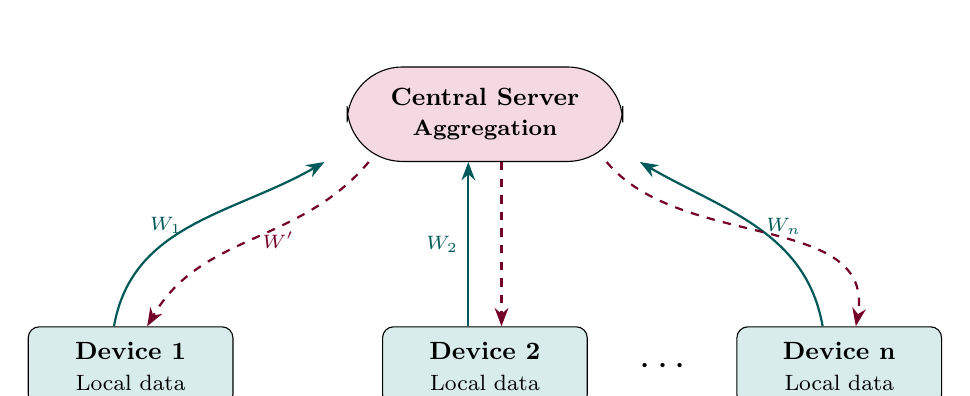
\begin{tikzpicture}[
  server/.style={rectangle, draw, rounded corners=20pt,
    fill=purple!15, minimum width=3.5cm, minimum height=1.2cm,
    font=\small\bfseries, align=center},
  client/.style={rectangle, draw, rounded corners=4pt,
    fill=teal!15, minimum width=2.6cm, minimum height=1.0cm,
    font=\small, align=center},
  up/.style={-{Stealth}, thick, color=teal!70!black},
  down/.style={-{Stealth}, thick, dashed, color=purple!60!black}
]
  \node[server] (S) at (0, 3.2)
    {\textbf{Central Server} \\ \footnotesize Aggregation};

  \node[client] (C1) at (-4.5, 0) {\textbf{Device 1} \\ \footnotesize Local data};
  \node[client] (C2) at (0,    0) {\textbf{Device 2} \\ \footnotesize Local data};
  \node[client] (C3) at (4.5,  0) {\textbf{Device n} \\ \footnotesize Local data};

  \node at (2.3, 0) {\Large $\cdots$};

  %% Upload: left side of each path going up
  \draw[up] ([xshift=-6pt]C1.north) to[out=80,in=210]
    node[midway, left, font=\scriptsize] {$W_1$}
    ([xshift=-8pt]S.south west);

  \draw[up] ([xshift=-6pt]C2.north) --
    node[midway, left, font=\scriptsize] {$W_2$}
    ([xshift=-6pt]S.south);

  \draw[up] ([xshift=-6pt]C3.north) to[out=100,in=330]
    node[midway, right, font=\scriptsize] {$W_n$}
    ([xshift=6pt]S.south east);

  %% Download: right side of each path going down
  \draw[down] ([xshift=8pt]S.south west) to[out=230,in=60]
    node[midway, right, font=\scriptsize] {$W'$}
    ([xshift=6pt]C1.north);

  \draw[down] ([xshift=6pt]S.south) --
    ([xshift=6pt]C2.north);

  \draw[down] ([xshift=-6pt]S.south east) to[out=310,in=80]
    ([xshift=6pt]C3.north);

\end{tikzpicture}
\caption{Standard Federated Learning Workflow}
\label{fig:fl-workflow}
\end{figure}
\vspace{\baselineskip}

The standard FL algorithm that implements this is Federated Averaging (FedAvg). It
is simple, well-understood, and works well under controlled conditions. However, it
has one structural problem that becomes critical in real-world deployments.

In FedAvg, the central server is not just a coordinator - it is the only entity
that can aggregate models and push the training forward. Every client must upload
to it, wait for it, and download from it every single round. This creates a hard
dependency: \textbf{if the server goes down at any point during training, every
client stops immediately}. There is no alternative path, no backup, and no way to
resume without restarting the server manually. In distributed systems, this kind of
dependency is called a \textbf{Single Point of Failure (SPOF)}.

In a research setting, this is manageable - if the server crashes, you restart
and try again. But in real-world FL deployments - hospitals sharing patient data
across branches, factories running FL across machines on a shop floor, or telecom
networks training models across hundreds of base stations - server downtime can
mean hours of lost training, corrupted experiment state, and no guarantee of
recovery. The larger the deployment, the more damaging an unexpected server failure
becomes.

The research community recognises this problem. Most major FL survey papers identify
the SPOF vulnerability of centralised architectures as one of the key barriers to
real-world adoption. The proposed solution is \textbf{decentralised FL} - where
nodes communicate directly with each other in a peer-to-peer network instead of
routing everything through a central server. If one node fails in such a setup,
the others can continue exchanging models and training without interruption. No
single node's failure can bring the entire system down.

This sounds like a clean solution, and theoretically it is. Convergence proofs
exist showing that decentralised gossip FL can match centralised FL performance
under ideal conditions. But here is the gap: \textbf{none of this has been tested
on real distributed infrastructure with live failure injection}. Every fault
tolerance claim in the decentralised FL literature is backed by either a
mathematical proof or a simulation. What actually happens when a server or node
is killed mid-experiment on real machines has never been directly measured and
reported.

This thesis fills that gap. It implements both a centralised FedAvg system and a
decentralised gossip FL system from scratch, deploys them on 8 real AWS EC2 cloud
instances, and runs controlled experiments covering normal training, live failure
injection, and a topology comparison between ring and fully-connected gossip graphs
-- to observe and measure the real outcome across all conditions.

\section{Contributions}

The specific contributions of this thesis are:

\begin{enumerate}
  \item A live demonstration of the SPOF problem in centralised FL on real cloud
  infrastructure, with timestamped log evidence from actual AWS EC2 instances -
  not a simulation.

  \item To the best of our knowledge, the first empirically measured
  accuracy-fault tolerance tradeoff between synchronous gossip FL and FedAvg
  under identical hardware and data conditions on real cloud infrastructure.

  \item Discovery of a cascading failure behaviour in synchronous ring gossip
  caused by TCP timeout propagation - an emergent real-world behaviour not described
  in any existing FL paper.

  \item A Non-IID sensitivity comparison between both architectures, with an
  explanation of why gossip FL degrades more under heterogeneous data.

  \item An empirical characterisation of how graph topology affects accuracy,
  convergence speed, and fault isolation scope in synchronous gossip FL: replacing
  the ring with a fully-connected graph increases accuracy by up to 8.50~pp and
  eliminates inter-node variance, but propagates node failures globally rather
  than locally.

  \item A complete open implementation of both architectures on 8 real AWS EC2
  instances with full experiment logs.
\end{enumerate}

\chapter{Literature Review}

This chapter surveys the existing work that directly leads to the research
question this thesis addresses. It covers the foundations of federated learning,
the challenges of non-IID data, the theoretical basis for decentralised FL, and
ends with the specific gap that remains unfilled in the literature.

\section{Federated Learning Foundations}

McMahan et al.~\cite{mcmahan2017} introduced Federated Averaging (FedAvg), which
remains the dominant FL algorithm. In FedAvg, a central server coordinates training
across clients - sending the global model out, collecting locally trained updates,
averaging them, and repeating. The key insight was that local SGD for multiple
epochs before aggregation is both communication-efficient and surprisingly effective.
FedAvg set the standard that all subsequent FL work builds on, and it is the
centralised baseline this thesis compares against.

Bonawitz et al.~\cite{bonawitz2019} studied FedAvg at scale and were among the
first to document the server's dual role as both a coordination hub and a
vulnerability. Their work identified that at production scale, the server becomes
a bottleneck and its failure has system-wide consequences - an early
acknowledgement of the SPOF problem that this thesis directly investigates.

\section{Non-IID Data in Federated Learning}

A key assumption in the original FedAvg paper is that data is identically
distributed across clients. In practice, this is almost never true. Each device
tends to have data skewed toward its own usage patterns - a user's phone sees
their photos, a hospital sees its patient population, a factory sees its own
machines. This is called \textbf{non-IID data}, and it creates a problem.

When data distributions differ across clients, locally trained models diverge from
each other during training. Averaging divergent models produces a global model that
does not represent any single client's data well. This phenomenon is called
\textbf{client drift}, and Li et al.~\cite{li2020} studied it formally, showing
that non-IID conditions cause FedAvg's convergence to slow significantly and final
accuracy to drop compared to the IID case. Their analysis motivates running
experiments under both data regimes - as this thesis does - to understand how
each architecture handles real-world data heterogeneity.

\section{Decentralised Federated Learning}

The theoretical case for decentralised FL was established by Lian et
al.~\cite{lian2017}, who proved that decentralised parallel SGD on a gossip
communication graph converges at the same asymptotic rate as centralised SGD
under certain conditions. This is a foundational result - it shows that
removing the central server does not necessarily hurt convergence, giving
theoretical credibility to the gossip-based approach.

Lalitha et al.~\cite{lalitha2019} proposed a fully decentralised FL framework
using gossip protocols, where each node exchanges models directly with a subset
of neighbours and aggregates locally. Their work demonstrated that gossip-based
FL can learn effectively without any central coordination, and they argued that
the peer-to-peer structure provides inherent fault tolerance - if one node
fails, the others simply continue. However, this fault tolerance claim was made
theoretically, without any real deployment or failure injection to validate it.

Boyd et al.~\cite{boyd2006} provided the mathematical foundations for gossip
algorithms on fixed network topologies. Their work on randomised gossip shows
how information spreads through a network and at what rate nodes converge
to a common value, with convergence speed determined by the graph's spectral
gap. This gives both topologies studied in this thesis -- the ring (minimum
spectral gap for a connected graph) and the fully-connected graph (maximum
spectral gap) -- a solid theoretical grounding. They represent the two extreme
points of the gossip connectivity spectrum.

Lian et al.~\cite{lian2017} extended this to the federated learning setting,
proving that decentralised parallel SGD converges at a rate that depends
directly on the graph's spectral gap. A higher spectral gap means faster
mixing and faster convergence -- the key theoretical prediction that the
topology comparison experiments in this thesis empirically test.

Tang et al.~\cite{tang2018} further showed that under heterogeneous (Non-IID)
data, higher graph connectivity provides a stronger corrective effect, because
nodes with diverse local distributions are more likely to be in direct contact.
This predicts that the accuracy gap between ring and fully-connected topologies
should be larger under Non-IID conditions than under IID -- a prediction
directly validated by the experiments in Chapter~\ref{ch:results}.

\subsection*{Positioning of Existing Work}
 
Table~\ref{tab:lit-comparison} summarises key decentralised FL papers
alongside this thesis. The gap is clear: no existing paper combines
real infrastructure deployment with controlled fault injection.
 
\begin{table}[H]
\centering
\small
\begin{tabular}{p{3.2cm}p{2.8cm}p{2.2cm}cc}
\toprule
\textbf{Work} & \textbf{Topology} & \textbf{Scale} &
\textbf{Real Infra?} & \textbf{Fault Tested?} \\
\midrule
Lian et al.~\cite{lian2017}             & General graph  & Simulation & No  & No \\
Lalitha et al.~\cite{lalitha2019}       & General gossip & Simulation & No  & No \\
Roy et al.~\cite{roy2019}               & P2P            & Simulation & No  & No \\
Beltran et al.~\cite{beltransurvey2023} & Survey         & N/A        & N/A & N/A \\
\textbf{This thesis} & \textbf{Ring + Fully Connected} & \textbf{8 AWS EC2} & \textbf{Yes} & \textbf{Yes} \\
\bottomrule
\end{tabular}
\vspace{0.5cm}
\caption{Comparison of decentralised FL works}
\label{tab:lit-comparison}
\end{table}

\section{The Gap This Thesis Fills}

Beltran et al.~\cite{beltransurvey2023} conducted one of the most comprehensive
surveys of decentralised FL to date. Their survey covers architectures, aggregation
strategies, fault tolerance mechanisms, and open challenges across dozens of papers.
A recurring observation in their survey is that decentralised FL is theoretically
mature but empirically underexplored - specifically, that fault tolerance is
argued for structurally but never actually demonstrated through live failure
experiments on real distributed infrastructure.

Kairouz et al.~\cite{kairouz2021} made a similar observation from a broader FL
perspective, noting that simulation-based evaluations dominate the field and that
real deployment behaviour - including failures, network variability, and hardware
differences - is rarely captured in published results.

Both surveys point to the same gap: the FL community lacks empirical evidence of
what decentralised FL actually does under real failure conditions, and how much
accuracy it sacrifices compared to centralised FedAvg when deployed on real
machines. This thesis is a direct response to that gap. It takes the architectures
that the literature has proposed and analysed theoretically, implements both from
scratch, runs them on real AWS EC2 infrastructure, and reports what actually
happens - including under deliberate, controlled failure injection that no
existing paper has performed on real hardware.

\section{Privacy Considerations in Federated Learning}

Federated Learning's foundational privacy property is that raw training data
never leaves each participating node. However, this does not make FL
unconditionally private. Zhu et al.~\cite{zhu2019} demonstrated that model
weight gradients can be used to reconstruct training samples with high fidelity
through gradient inversion, showing that model updates themselves are an
information channel. Fredrikson et al.~\cite{fredrikson2015} further showed that
model parameters alone can be exploited via model inversion attacks to recover
class-representative inputs.

Differential Privacy (DP), formalised by Dwork et al.~\cite{dwork2006}, provides
the strongest formal guarantee against such leakage: it bounds the information
an adversary can infer about any individual training example from the output of
a computation. Geyer et al.~\cite{geyer2017} applied DP to the FL setting by
clipping each client's gradient update and adding calibrated Gaussian noise
before server aggregation, providing per-client privacy at a measurable accuracy
cost.

This thesis does not implement Differential Privacy. Adding calibrated noise to
model updates would alter the accuracy baseline and make it impossible to
attribute observed accuracy differences solely to architectural topology -
the primary variable under investigation. DP integration in gossip-based FL,
where noise budgets must be managed without a central aggregator, remains an
open direction for future work.

\section{Convergence Analysis Under Heterogeneous Data}

The convergence impact of non-IID data on FedAvg has been formally characterised
in the literature. Li et al.~\cite{li2020} showed that client drift - the
divergence of locally trained models from the global optimum under heterogeneous
data - causes FedAvg's convergence to slow and final accuracy to drop compared
to the IID case. Two algorithmic responses have been proposed. FedProx~\cite{li2020}
adds a proximal term to each client's local objective that penalises deviations
from the current global model, limiting the extent of local drift.
SCAFFOLD~\cite{karimireddy2020} uses control variates to correct the gradient
direction at each client, reducing drift without restricting the number of local
training steps.

Analogous corrections for decentralised gossip settings are less developed.
Tang et al.~\cite{tang2018} studied gradient tracking in decentralised
optimisation over decentralised data, showing that tracking local gradient
estimates can correct for network-induced bias in the aggregation. Whether
these corrections carry over cleanly to synchronous ring gossip FL under
Non-IID conditions - where each node's aggregation neighbourhood is fixed
and small - remains an open question. This thesis contributes an empirical
data point by quantifying the Non-IID sensitivity gap between centralised
FedAvg and ring gossip FL under identical experimental conditions.

\chapter{Problem Formulation}

\section{Problem Statement}

As established in the previous chapters, centralised federated learning has a
well-known architectural weakness - everything depends on the central server.
The research community has proposed decentralised FL as the solution, where nodes
communicate directly in a peer-to-peer network. The theoretical case is strong:
no central server means no single point of failure, and convergence proofs show
that gossip-based FL can match centralised performance under ideal conditions.

But theory and simulation are not the same as real deployment. Real machines
fail unexpectedly. Real networks behave differently from simulated ones. Real
TCP connections time out. None of the existing decentralised FL papers have
actually deployed both architectures on real infrastructure, injected failures,
and measured what happens.

This thesis addresses that directly. The central research question is:

\vspace{0.3cm}
\textit{How does decentralised synchronous gossip FL compare to centralised
FedAvg in terms of model accuracy, communication behaviour, and fault tolerance
-- when both are deployed on real cloud infrastructure under identical
conditions, including under live failure injection? And within decentralised
FL, how does graph topology shape these properties?}
\vspace{0.3cm}

\section{Research Questions}

The central question above breaks down into five specific questions that the
experiments in this thesis are designed to answer.

\textbf{RQ1: Does decentralised gossip FL achieve comparable accuracy to
centralised FedAvg?}

Removing the central server changes how models are aggregated. In centralised
FL, every client's model is averaged together in one step. In gossip FL, each
node only blends with its two immediate neighbours, and knowledge spreads
gradually across the ring. This raises the question of whether this local
blending is good enough to reach the same accuracy as global averaging. We test
this under both IID and Non-IID data conditions, since the answer may differ
depending on how similar or different the data across nodes is.

\textbf{RQ2: How does each architecture behave under Non-IID data?}

In practice, data across FL nodes is rarely uniform. Each node tends to have
data skewed toward certain patterns - a hospital sees certain patient types,
a factory sees certain machine readings. This non-IID condition is known to hurt
FL accuracy. The question is whether it hurts both architectures equally, or
whether the smaller aggregation pool in gossip FL (2 neighbours vs.\ all 7
clients) makes it more sensitive to data heterogeneity.

\textbf{RQ3: What actually happens when a critical node fails during training?}

This is the core fault tolerance question. In centralised FL, the server failing
should halt all clients - but by exactly how much, for exactly how long, and
with what final accuracy impact? In decentralised FL, a node failing should allow
others to continue - but does the ring recover cleanly, or are there secondary
effects? We answer this by deliberately killing the server (centralised) and one
ring node (decentralised) mid-experiment on real AWS infrastructure and observing
the outcome in both cases.

\textbf{RQ4: Are there failure behaviours in ring gossip that theory does not
predict?}

Theoretical gossip models assume clean message passing - a node either sends
its model successfully or it does not. Real TCP communication is more complex.
Timeouts, retries, and synchronisation delays can create second-order effects
that simple theoretical models miss. This question asks whether deploying on
real infrastructure reveals any such behaviours.

\textbf{RQ5: How does graph topology affect accuracy, convergence, and fault
tolerance in decentralised FL?}

The ring topology used in Experiments 1--4 is the standard gossip baseline,
but it is also the sparsest connected graph. A fully-connected graph, where
every node communicates with every other node, represents the opposite extreme.
Both graphs are well-studied theoretically -- they have the lowest and highest
possible spectral gaps, respectively -- but their comparative behaviour on real
infrastructure under both normal and fault conditions has not been measured.
This question asks what accuracy, convergence, and fault isolation properties
each topology produces in practice, and whether the theoretical predictions
hold on real distributed hardware.

\section{Design Decisions}

Two design choices were made deliberately to ensure the comparison is fair and
interpretable.

\textbf{Synchronous protocol for both architectures.} In a synchronous protocol,
every node waits for its partners to finish before proceeding to the next round.
Using async on one side would introduce model staleness as a second variable on
top of topology, making it impossible to attribute any accuracy difference to
topology alone. Keeping both sides synchronous means the only thing that differs
between the two systems is whether there is a central server or not.

\textbf{Ring topology as the primary decentralised baseline.} Each node in the
ring connects to exactly two neighbours -- the node to its left and to its right.
This is the standard baseline gossip topology in the literature~\cite{boyd2006},
well-understood in terms of how information propagates and how the spectral gap
governs convergence speed. It is the right choice for the primary comparison
against centralised FedAvg, as it isolates the effect of decentralisation itself
without introducing additional connectivity variables.

\textbf{Fully-connected topology as the upper bound.} Once the ring baseline is
established, replacing the ring with a fully-connected graph -- where every node
communicates with all others -- isolates the effect of graph topology within the
decentralised setting. These two topologies represent the lowest and highest
possible spectral gaps for a connected graph, making them the natural pair of
endpoints for a topology comparison study.

\section{Scope and Limitations}

This thesis focuses on synchronous FL with 8 nodes, comparing centralised FedAvg
against decentralised gossip FL under two topologies: ring and fully-connected.
It does not address asynchronous FL, intermediate or dynamic topologies, Byzantine
fault tolerance, or large-scale deployments beyond 8 nodes. These are all valid
research directions but are explicitly out of scope here -- the goal is a clean,
controlled comparison across the two extreme points of gossip connectivity, not a
comprehensive survey of all possible graph configurations. Scaling behaviour,
adaptive timeout mechanisms, and intermediate topology designs are left as
directions for future work.

\chapter{System Design and Architecture}

This chapter describes the design of the two federated learning systems built
for this thesis - a centralised FedAvg system and a decentralised gossip FL
system. Both were implemented from scratch in Python and PyTorch using raw TCP
socket communication, and deployed on real AWS EC2 instances.

\section{Centralised FedAvg Architecture}

The centralised system follows the standard FedAvg design. One node acts as the
server and the remaining seven act as clients, forming a star topology where all
communication passes through the server.

Each training round proceeds in three steps. First, the server opens a listener
and waits to receive locally trained models from all seven clients. Once all
models arrive, it computes a simple average - equal weight for each client -
and produces an updated global model. Finally, it broadcasts this global model
back to all clients, and the next round begins.

Communication uses two TCP ports on the server: one for clients to upload their
models, and one for the server to broadcast the aggregated model back. Each model
is serialised using PyTorch's \texttt{torch.save} and sent as raw bytes over the
socket. The server waits for all seven clients before aggregating - no client
can proceed to the next round until the server has received from everyone and
broadcast the result.

This synchronous, server-centric design is exactly the standard FedAvg setup
described in McMahan et al.~\cite{mcmahan2017}. It serves as the baseline against
which the decentralised system is compared.

\begin{figure}[ht]
\centering
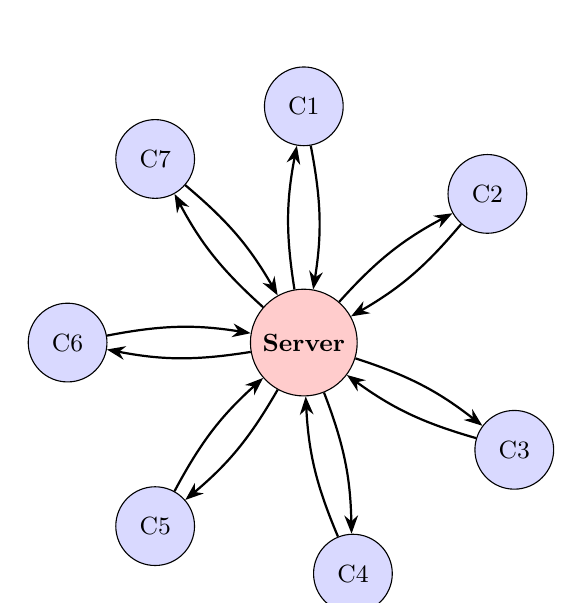
\begin{tikzpicture}[
  server/.style={circle, draw=black, fill=red!20, minimum size=1.2cm, font=\small\bfseries},
  client/.style={circle, draw=black, fill=blue!15, minimum size=1cm, font=\small},
  arr/.style={-{Stealth}, thick}
]
  \node[server] (S) at (0,0) {Server};
  \foreach \i/\angle in {1/90, 2/39, 3/333, 4/282, 5/231, 6/180, 7/129}{
    \node[client] (C\i) at (\angle:3cm) {C\i};
    \draw[arr, bend left=10] (S) to (C\i);
    \draw[arr, bend left=10] (C\i) to (S);
  }
\end{tikzpicture}
\caption{Centralised FedAvg - Star Topology (1 Server + 7 Clients)}
\label{fig:centralised-arch}
\end{figure}

The structural consequence of this design is clear: the server is the only entity
that can move training forward. If it fails, all clients are left waiting
indefinitely with no recovery path.

\section{Decentralised Gossip FL Architecture}

The decentralised system eliminates the server entirely. All 8 nodes are equal
peers arranged in a fixed ring topology, where each node is connected only to its
immediate left and right neighbours.

Each training round proceeds in three steps as well, but the logic is local to
each node. First, every node trains independently on its local data for a fixed
number of epochs. Then, each node simultaneously pushes its trained model to both
neighbours and receives models from both neighbours - this exchange is
bidirectional and happens in parallel across the ring. Finally, each node blends
the three models it now holds (its own plus the two received) using equal-weight
averaging, evaluates the blended model, and waits for the next round to begin.

Communication uses one TCP port per node. Each node opens a listener for incoming
models and connects outward to push its model to both neighbours. If a push fails
- because the neighbour is temporarily unavailable - the node retries for up
to 90 seconds before giving up and continuing with whatever models it has received.
This retry mechanism is what creates the timing effects observed in the fault
tolerance experiments.

\begin{figure}[ht]
\centering
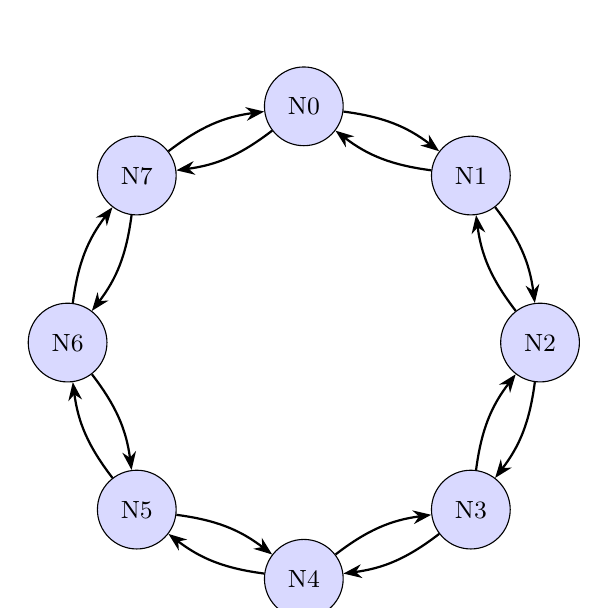
\begin{tikzpicture}[
  node/.style={circle, draw=black, fill=blue!15, minimum size=1cm, font=\small},
  arr/.style={-{Stealth}, thick}
]
  \foreach \i/\angle in {0/90, 1/45, 2/0, 3/315, 4/270, 5/225, 6/180, 7/135}{
    \node[node] (N\i) at (\angle:3cm) {N\i};
  }
  \foreach \i/\j in {0/1, 1/2, 2/3, 3/4, 4/5, 5/6, 6/7, 7/0}{
    \draw[arr, bend left=15] (N\i) to (N\j);
    \draw[arr, bend left=15] (N\j) to (N\i);
  }
\end{tikzpicture}
\caption{Decentralised Gossip FL - Ring Topology (8 Peer Nodes)}
\label{fig:decentralised-arch}
\end{figure}

Because no node plays a special role, no single node's failure can halt the
system. The remaining nodes continue exchanging with their surviving neighbours
and completing training rounds independently.

\section{Fully-Connected Gossip Architecture}

A second decentralised configuration extends the ring design by replacing the
ring graph with a fully-connected graph. Every node communicates directly with
all other nodes each round, rather than only its two ring neighbours.

The per-round protocol is identical in structure: train locally, push the
trained model to all peers simultaneously using concurrent outbound connections,
receive models from all peers, blend, and evaluate. The blend pool expands from
three models (self plus two ring neighbours) to eight models (self plus all seven
peers), which is mathematically equivalent to computing a global average without
a central server.

The key structural difference from the ring is that every node holds a direct
edge to every other node. This means that information from any node reaches all
other nodes in a single round (diameter~1), whereas in the ring it takes up to
four hops. Under fault conditions, this same property means that any single
node failure is immediately visible to all surviving nodes, whereas in the ring
only the two direct neighbours are directly affected.

\begin{figure}[ht]
\centering
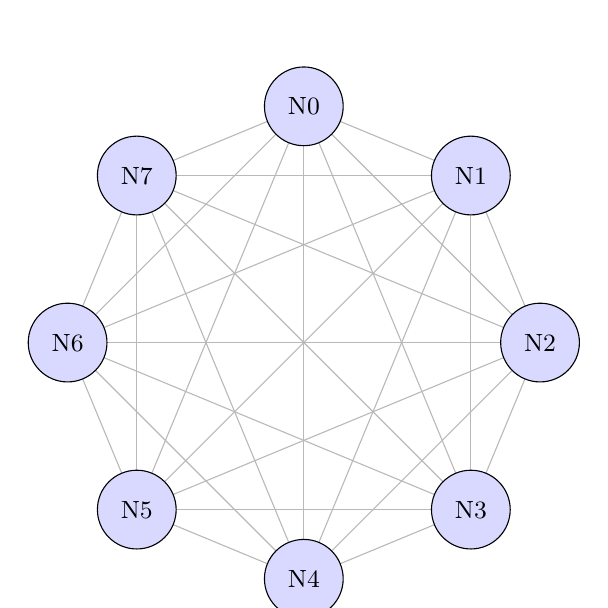
\begin{tikzpicture}[
  fnode/.style={circle, draw=black, fill=blue!15, minimum size=1cm, font=\small},
  conn/.style={gray!55, thin}
]
  % Place all 28 edges behind the nodes
  \foreach \i in {0,...,7}{
    \coordinate (P\i) at ({90 - \i*45}:3cm);
  }
  \foreach \i in {0,...,7}{
    \foreach \j in {0,...,7}{
      \pgfmathtruncatemacro{\cond}{(\j > \i) ? 1 : 0}
      \ifnum\cond=1
        \draw[conn] (P\i) -- (P\j);
      \fi
    }
  }
  % Draw nodes on top of the edges
  \foreach \i/\angle in {0/90, 1/45, 2/0, 3/315, 4/270, 5/225, 6/180, 7/135}{
    \node[fnode] (N\i) at (\angle:3cm) {N\i};
  }
\end{tikzpicture}
\caption{Decentralised Gossip FL -- Fully-Connected Topology (8 Peer Nodes, 28 bidirectional links)}
\label{fig:fc-arch}
\end{figure}

This fully-connected configuration serves as the upper bound of gossip
connectivity in this thesis, paired with the ring as the lower bound.

\section{Design Comparison}

\begin{table}[ht]
\centering
\begin{tabular}{llll}
\toprule
\textbf{Property} & \textbf{Centralised FedAvg} & \textbf{Ring Gossip} & \textbf{Fully Connected} \\
\midrule
Topology          & Star (1 server + 7 clients) & Ring (degree~2)       & Complete (degree~7) \\
Aggregation       & Global average at server    & Blend: self + 2 peers & Blend: self + all 7 \\
Communication     & All clients $\to$ server    & $\leftrightarrow$ 2 neighbours & $\leftrightarrow$ all 7 peers \\
Spectral gap      & N/A                         & Low ($\approx$0.19)   & Maximum (1.0) \\
Knowledge spread  & Instant (1 round)           & Gradual (ring hops)   & Instant (1 hop) \\
SPOF              & Yes (server)                & No                    & No \\
Fault scope       & System-wide halt            & 2 neighbours affected & All nodes affected \\
Failure recovery  & None                        & Continues locally     & Continues; globally slowed \\
\bottomrule
\end{tabular}
\vspace{0.5cm}
\caption{Architecture and topology comparison}
\label{tab:design-comparison}
\end{table}

The table reveals a three-way set of trade-offs. Centralised FedAvg spreads
knowledge instantly across all clients in one round, but introduces a single
point of failure. Ring gossip eliminates the SPOF and contains fault impact to
direct neighbours, but propagates knowledge slowly across hops -- the primary
reason it achieves lower accuracy than FedAvg, an effect that grows more
significant under Non-IID data. Fully-connected gossip closes most of the
accuracy gap by giving every node immediate access to all peers' models each
round, and eliminates inter-node accuracy variance entirely; however, it
trades the ring's localised fault containment for global fault propagation,
where any single node failure is simultaneously visible to all surviving nodes.

\section{Infrastructure}

Both systems were deployed on AWS EC2 t3.micro instances running Ubuntu
22.04, all within the same VPC and subnet. Nodes communicate over the private
subnet using their internal IP addresses. Each instance runs one FL process -
either the server or a client in the centralised case, or one ring node in the
decentralised case. No FL framework was used; both systems were implemented
entirely from scratch using Python sockets and PyTorch.

\section{Communication Protocol Detail}
 
\begin{figure}[H]
\centering
\resizebox{0.82\textwidth}{!}{%
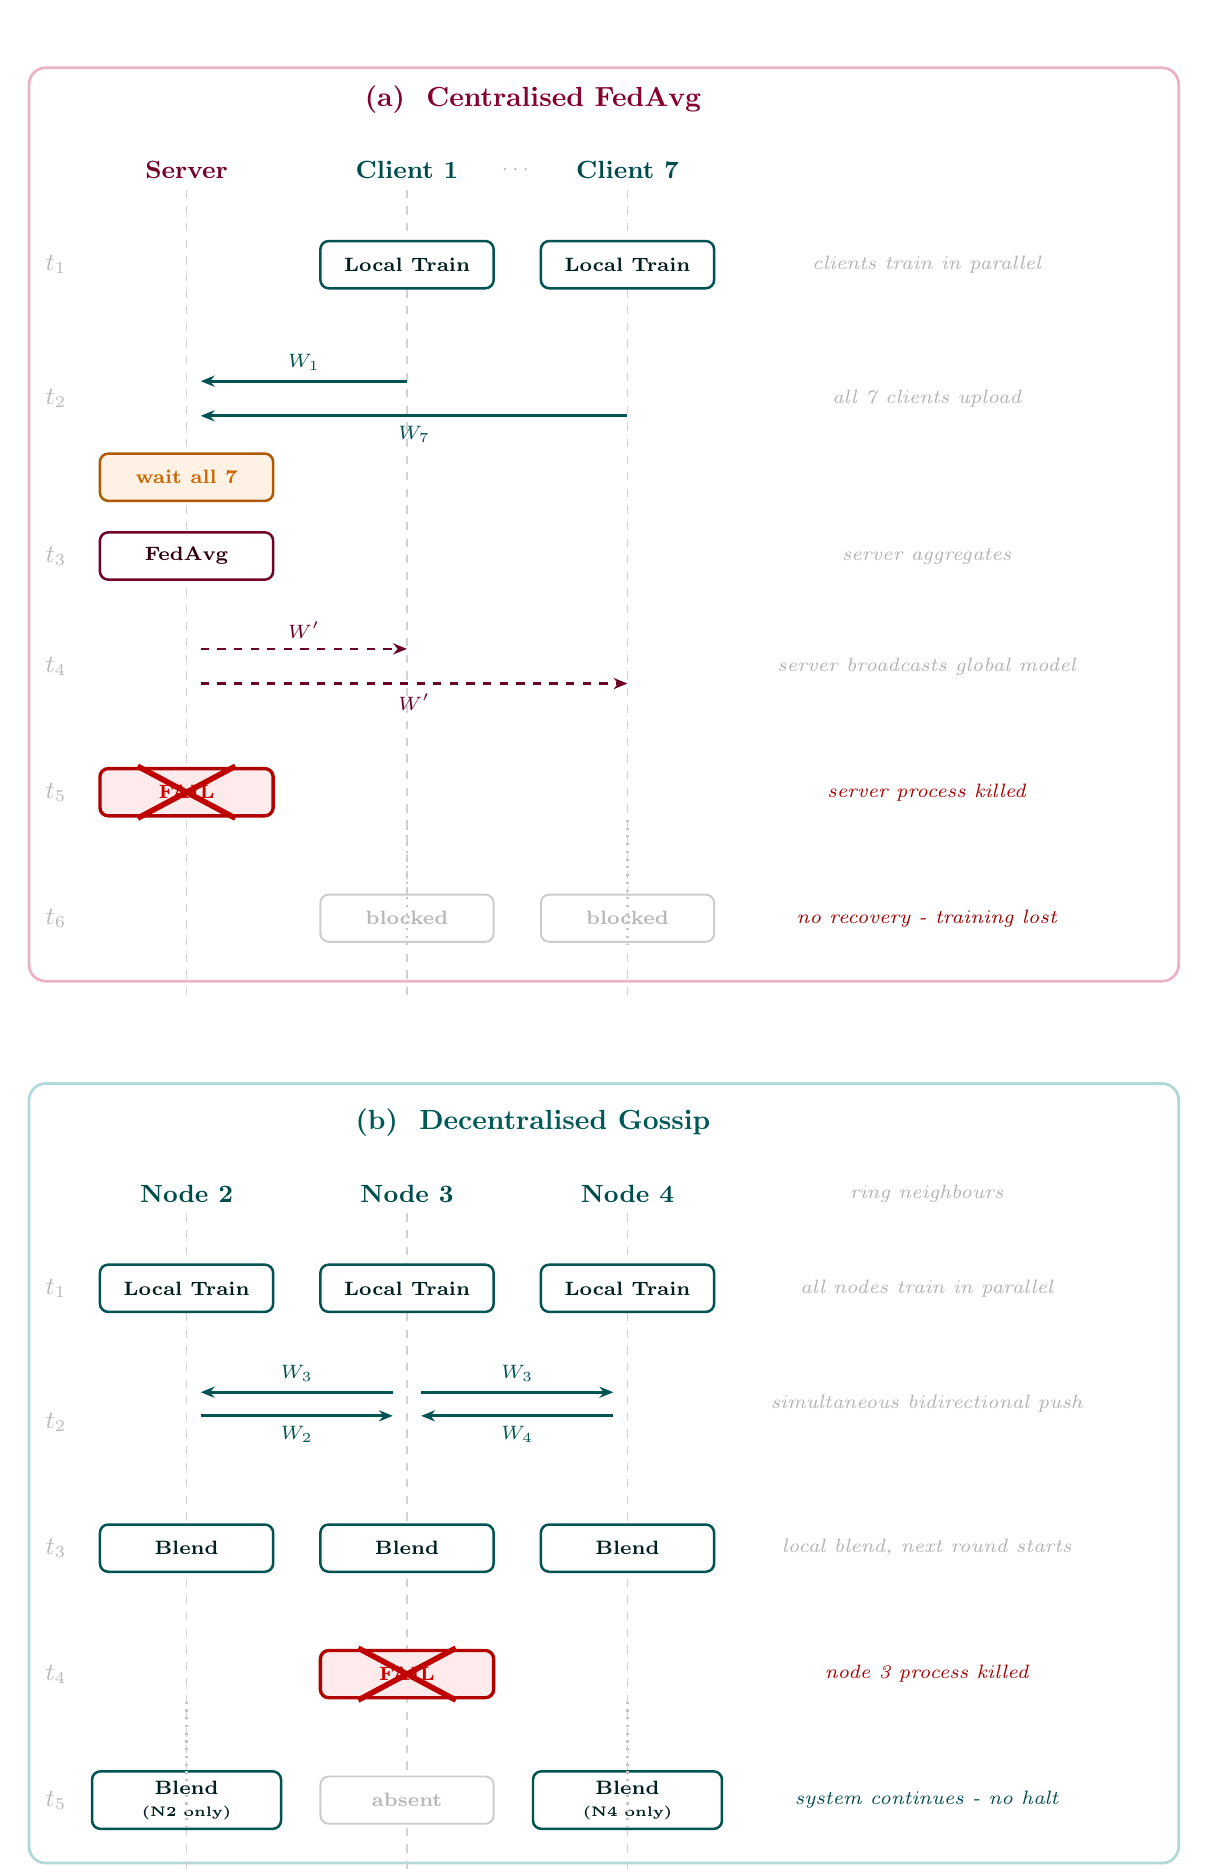
\begin{tikzpicture}[
  clientbox/.style={
    rectangle, rounded corners=3pt,
    minimum width=2.2cm, minimum height=0.6cm,
    font=\scriptsize\bfseries, align=center,
    fill=white, draw=teal!65!black, line width=0.9pt,
    text=teal!25!black},
  serverbox/.style={
    rectangle, rounded corners=3pt,
    minimum width=2.2cm, minimum height=0.6cm,
    font=\scriptsize\bfseries, align=center,
    fill=white, draw=purple!60!black, line width=0.9pt,
    text=purple!25!black},
  failbox/.style={
    rectangle, rounded corners=3pt,
    minimum width=2.2cm, minimum height=0.6cm,
    font=\scriptsize\bfseries, align=center,
    fill=red!8, draw=red!70!black, line width=1.2pt,
    text=red!80!black},
  blockedbox/.style={
    rectangle, rounded corners=3pt,
    minimum width=2.2cm, minimum height=0.6cm,
    font=\scriptsize\bfseries, align=center,
    fill=white, draw=gray!40, line width=0.7pt,
    text=gray!55},
  barrier/.style={
    rectangle, rounded corners=3pt,
    minimum width=2.2cm, minimum height=0.6cm,
    font=\scriptsize\bfseries, align=center,
    fill=orange!10, draw=orange!70!black, line width=0.9pt,
    text=orange!80!black},
  lifeline/.style={gray!35, dashed, line width=0.6pt},
  uparrow/.style={
    -{Stealth[length=5pt,width=4pt]},
    line width=1.0pt, color=teal!65!black},
  downarrow/.style={
    -{Stealth[length=5pt,width=4pt]},
    line width=1.0pt, dashed, color=purple!55!black},
  pusharrow/.style={
    -{Stealth[length=5pt,width=4pt]},
    line width=1.0pt, color=teal!65!black},
  dotline/.style={gray!45, line width=0.8pt, dotted},
  timelabel/.style={
    font=\small\bfseries, text=gray!55, anchor=east},
  headerlabel/.style={font=\small\bfseries},
  annot/.style={font=\scriptsize\itshape, text=gray!60},
  paneltitle/.style={font=\normalsize\bfseries},
]

%% ============================================================
%% COLUMN X-POSITIONS
%% ============================================================
\def\Tleft{1.6}   % left margin for time labels
\def\Tsrv{3.0}    % Server / Node 2
\def\Tca{5.8}     % Client 1 / Node 3
\def\Tcb{8.6}     % Client 7 / Node 4
\def\Tannot{12.4} % annotation column — shifted right
\def\Tright{15.6} % right edge of panel — wider

%% ============================================================
%% TOP PANEL Y-POSITIONS
%% ============================================================
\def\Utitle{0.6}
\def\Uhead{-0.3}
\def\Ua{-1.5}
\def\Ub{-3.2}
\def\Ubar{-4.2}
\def\Uc{-5.2}
\def\Ud{-6.6}
\def\Ue{-8.2}
\def\Uf{-9.8}
\def\Ubot{-11.0}

%% ============================================================
%% BOTTOM PANEL Y-POSITIONS
%% ============================================================
\def\Dtitle{-12.4}
\def\Dhead{-13.3}
\def\Da{-14.5}
\def\Db{-16.2}
\def\Dc{-17.8}
\def\De{-19.4}
\def\Df{-21.0}
\def\Dbot{-22.2}

%% ============================================================
%% PANEL OUTLINES
%% ============================================================
\draw[purple!30, rounded corners=6pt, line width=1.0pt]
  (1.0, 1.0) rectangle (\Tright, \Ubot+0.4);

\draw[teal!30, rounded corners=6pt, line width=1.0pt]
  (1.0, \Dtitle+0.5) rectangle (\Tright, \Dbot+0.4);

%% ============================================================
%% TOP PANEL — CENTRALISED FEDAVG
%% ============================================================

\node[paneltitle, text=purple!70!black]
  at (7.4, \Utitle) {(a)~~Centralised FedAvg};

%% Column headers
\node[headerlabel, text=purple!60!black]
  at (\Tsrv, \Uhead) {Server};
\node[headerlabel, text=teal!60!black]
  at (\Tca, \Uhead) {Client 1};
\node[annot] at (7.2, \Uhead) {$\cdots$};
\node[headerlabel, text=teal!60!black]
  at (\Tcb, \Uhead) {Client 7};

%% Lifelines
\draw[lifeline] (\Tsrv, \Uhead-0.25) -- (\Tsrv, \Ubot+0.2);
\draw[lifeline] (\Tca,  \Uhead-0.25) -- (\Tca,  \Ubot+0.2);
\draw[lifeline] (\Tcb,  \Uhead-0.25) -- (\Tcb,  \Ubot+0.2);

%% Time labels
\node[timelabel] at (\Tleft, \Ua) {$t_1$};
\node[timelabel] at (\Tleft, \Ub) {$t_2$};
\node[timelabel] at (\Tleft, \Uc) {$t_3$};
\node[timelabel] at (\Tleft, \Ud) {$t_4$};
\node[timelabel] at (\Tleft, \Ue) {$t_5$};
\node[timelabel] at (\Tleft, \Uf) {$t_6$};

%% t1 — Local Training
\node[clientbox] at (\Tca, \Ua) {Local Train};
\node[clientbox] at (\Tcb, \Ua) {Local Train};
\node[annot] at (\Tannot, \Ua)
  {\textit{clients train in parallel}};

%% t2 — Upload arrows
\draw[uparrow]
  (\Tca, \Ub+0.22) --
  node[above, font=\scriptsize\bfseries,
    text=teal!65!black]{$W_1$}
  (\Tsrv+0.18, \Ub+0.22);
\draw[uparrow]
  (\Tcb, \Ub-0.22) --
  node[below, font=\scriptsize\bfseries,
    text=teal!65!black]{$W_7$}
  (\Tsrv+0.18, \Ub-0.22);
\node[annot] at (\Tannot, \Ub)
  {\textit{all 7 clients upload}};

%% Barrier
\node[barrier] at (\Tsrv, \Ubar) {wait all 7};

%% t3 — FedAvg
\node[serverbox] at (\Tsrv, \Uc) {FedAvg};
\node[annot] at (\Tannot, \Uc)
  {\textit{server aggregates}};

%% t4 — Broadcast
\draw[downarrow]
  (\Tsrv+0.18, \Ud+0.22) --
  node[above, font=\scriptsize\bfseries,
    text=purple!55!black]{$W'$}
  (\Tca, \Ud+0.22);
\draw[downarrow]
  (\Tsrv+0.18, \Ud-0.22) --
  node[below, font=\scriptsize\bfseries,
    text=purple!55!black]{$W'$}
  (\Tcb, \Ud-0.22);
\node[annot] at (\Tannot, \Ud)
  {\textit{server broadcasts global model}};

%% t5 — Server FAIL
\node[failbox] at (\Tsrv, \Ue) {\textbf{FAIL}};
\draw[red!75!black, line width=2.0pt]
  (\Tsrv-0.62, \Ue+0.33) -- (\Tsrv+0.62, \Ue-0.33);
\draw[red!75!black, line width=2.0pt]
  (\Tsrv+0.62, \Ue+0.33) -- (\Tsrv-0.62, \Ue-0.33);
\node[annot, text=red!65!black] at (\Tannot, \Ue)
  {\textit{server process killed}};

%% t6 — Blocked
\node[blockedbox] at (\Tca, \Uf) {blocked};
\node[blockedbox] at (\Tcb, \Uf) {blocked};
\draw[dotline] (\Tca, \Ue-0.35) -- (\Tca, \Uf-0.33);
\draw[dotline] (\Tcb, \Ue-0.35) -- (\Tcb, \Uf-0.33);
\node[annot, text=red!60!black] at (\Tannot, \Uf)
  {\textit{no recovery - training lost}};

%% ============================================================
%% BOTTOM PANEL — DECENTRALISED GOSSIP
%% ============================================================

\node[paneltitle, text=teal!70!black]
  at (7.4, \Dtitle) {(b)~~Decentralised Gossip};

%% Column headers
\node[headerlabel, text=teal!60!black]
  at (\Tsrv, \Dhead) {Node 2};
\node[headerlabel, text=teal!60!black]
  at (\Tca,  \Dhead) {Node 3};
\node[headerlabel, text=teal!60!black]
  at (\Tcb,  \Dhead) {Node 4};
\node[annot] at (\Tannot, \Dhead)
  {\textit{ring neighbours}};

%% Lifelines
\draw[lifeline] (\Tsrv, \Dhead-0.25) -- (\Tsrv, \Dbot+0.2);
\draw[lifeline] (\Tca,  \Dhead-0.25) -- (\Tca,  \Dbot+0.2);
\draw[lifeline] (\Tcb,  \Dhead-0.25) -- (\Tcb,  \Dbot+0.2);

%% Time labels
\node[timelabel] at (\Tleft, \Da) {$t_1$};
\node[timelabel] at (\Tleft, \Db) {$t_2$};
\node[timelabel] at (\Tleft, \Dc) {$t_3$};
\node[timelabel] at (\Tleft, \De) {$t_4$};
\node[timelabel] at (\Tleft, \Df) {$t_5$};

%% t1 — Local Training
\node[clientbox] at (\Tsrv, \Da) {Local Train};
\node[clientbox] at (\Tca,  \Da) {Local Train};
\node[clientbox] at (\Tcb,  \Da) {Local Train};
\node[annot] at (\Tannot, \Da)
  {\textit{all nodes train in parallel}};

%% t2 — Bidirectional push
%% N3 -> N2
\draw[pusharrow]
  (\Tca-0.18, \Db+0.38) --
  node[above, font=\scriptsize\bfseries,
    text=teal!65!black]{$W_3$}
  (\Tsrv+0.18, \Db+0.38);
%% N2 -> N3
\draw[pusharrow]
  (\Tsrv+0.18, \Db+0.08) --
  node[below, font=\scriptsize\bfseries,
    text=teal!65!black]{$W_2$}
  (\Tca-0.18, \Db+0.08);
%% N3 -> N4
\draw[pusharrow]
  (\Tca+0.18, \Db+0.38) --
  node[above, font=\scriptsize\bfseries,
    text=teal!65!black]{$W_3$}
  (\Tcb-0.18, \Db+0.38);
%% N4 -> N3
\draw[pusharrow]
  (\Tcb-0.18, \Db+0.08) --
  node[below, font=\scriptsize\bfseries,
    text=teal!65!black]{$W_4$}
  (\Tca+0.18, \Db+0.08);
\node[annot] at (\Tannot, \Db+0.23)
  {\textit{simultaneous bidirectional push}};

%% t3 — Blend (normal round)
\node[clientbox] at (\Tsrv, \Dc) {Blend};
\node[clientbox] at (\Tca,  \Dc) {Blend};
\node[clientbox] at (\Tcb,  \Dc) {Blend};
\node[annot] at (\Tannot, \Dc)
  {\textit{local blend, next round starts}};

%% t4 — Node 3 FAIL
\node[failbox] at (\Tca, \De) {\textbf{FAIL}};
\draw[red!75!black, line width=2.0pt]
  (\Tca-0.62, \De+0.33) -- (\Tca+0.62, \De-0.33);
\draw[red!75!black, line width=2.0pt]
  (\Tca+0.62, \De+0.33) -- (\Tca-0.62, \De-0.33);
\node[annot, text=red!65!black] at (\Tannot, \De)
  {\textit{node 3 process killed}};

%% t5 — Neighbours continue with reduced blend
\node[clientbox, minimum width=2.4cm] at (\Tsrv, \Df)
  {Blend\\{\tiny (N2 only)}};
\node[blockedbox] at (\Tca, \Df) {absent};
\node[clientbox, minimum width=2.4cm] at (\Tcb, \Df)
  {Blend\\{\tiny (N4 only)}};
\draw[dotline] (\Tsrv, \De-0.35) -- (\Tsrv, \Df-0.33);
\draw[dotline] (\Tcb,  \De-0.35) -- (\Tcb,  \Df-0.33);
\node[annot, text=teal!60!black] at (\Tannot, \Df)
  {\textit{system continues - no halt}};

\end{tikzpicture}%
}% end resizebox

\caption{Round execution timeline for one training round in each
architecture (time flows downward).
\textbf{(a) Centralised FedAvg:} Steps are strictly sequential -
local training ($t_1$), all-client upload ($t_2$), server
aggregation ($t_3$), broadcast ($t_4$). A server failure at $t_5$
permanently blocks every client with no recovery path.
\textbf{(b) Decentralised Gossip:} Local training ($t_1$),
bidirectional push ($t_2$), and local blend ($t_3$) all proceed
in parallel. A node failure at $t_4$ is absorbed by neighbours
who continue with a reduced blend at $t_5$ - the system never halts.}
\label{fig:comm-sequence}
\end{figure}
 
In the centralised system, each round involves two sequential network
phases: all clients upload, then the server broadcasts. In the
decentralised system, both push and receive happen in parallel across
the ring - each node pushes to two neighbours and receives from two
neighbours simultaneously. This parallel exchange is why gossip
communication time is dominated by neighbour training speed rather
than network bandwidth.
 
Model serialisation in both systems uses PyTorch's \texttt{state\_dict}
serialised with \texttt{torch.save} to a byte buffer, transmitted
as raw bytes over TCP. The serialised CNNCifar model is consistently
245.3~KB per transfer. No compression or differential encoding is used
- the full model is exchanged every round.

\chapter{Experimental Methodology}

This chapter describes the experimental setup used to compare the two
architectures. It covers the infrastructure, the model and dataset, the
data distribution conditions, and the nine experiments that were run.

\section{Infrastructure}

Both architectures were deployed on \textbf{8 AWS EC2 t3.micro instances},
each running Ubuntu 22.04. All instances were placed within the same Virtual
Private Cloud (VPC) and subnet, communicating over private IP addresses. Each
instance ran a single FL process - either the server or a client in the
centralised setup, or one peer node in the decentralised setup (ring or
fully-connected, depending on the experiment).

No FL framework was used. Both systems were implemented from scratch in Python
using raw TCP sockets and PyTorch. This was a deliberate choice - using a
framework would abstract away the network behaviour and make it harder to observe
real failure effects.

\section{Model and Dataset}

All experiments used \textbf{CIFAR-10}, a standard image classification dataset
with 50,000 training images and 10,000 test images across 10 classes. The model
was a simple CNN (referred to as CNNCifar) with two convolutional layers followed
by two fully connected layers, totalling approximately 62,000 parameters. The
serialised model size was 245.3 KB per exchange.

CIFAR-10 was chosen because it is a well-established FL benchmark, large enough
to show meaningful accuracy differences across data distributions, and small
enough to run efficiently on t3.micro instances without GPU acceleration.

\section{Data Distribution}

Each experiment was run under two data distribution conditions.

\textbf{IID} - the 50,000 training images were split randomly and uniformly
across all 7 clients (centralised) or 8 nodes (decentralised), giving each
participant roughly 6,250 samples with balanced class representation. This is
the ideal case where all participants see similar data.

\textbf{Non-IID} - data was distributed using a \textbf{Dirichlet distribution
with $\alpha = 0.5$}. This causes each participant to receive a skewed sample
dominated by only a few classes, making local models diverge during training.
This is closer to real-world FL deployments where each device naturally sees
only the data relevant to its own context. The value $\alpha = 0.5$ represents
moderate heterogeneity - severe enough to meaningfully stress-test both
architectures, but not so extreme as to make learning practically impossible.

\section{Hyperparameters}

The following hyperparameters were kept identical across all nine experiments to
ensure a fair comparison between the two architectures.

\begin{table}[H]
\centering
\caption{Hyperparameters used across all experiments}
\label{tab:hyperparams}
\begin{tabular}{ll}
\toprule
\textbf{Parameter} & \textbf{Value} \\
\midrule
FL rounds          & 50 \\
Local epochs       & 5 \\
Batch size         & 64 \\
Optimiser          & SGD (no momentum) \\
Learning rate      & 0.01 \\
Inter-round sleep  & 5 seconds \\
\bottomrule
\end{tabular}
\end{table}

\section{Pilot Study}

Before the main AWS experiments, a two-node pilot study was conducted on two
VMware virtual machines connected over a bridged local network. This pilot
confirmed that the P2P TCP communication infrastructure worked correctly across
real machines, and produced an unplanned server crash at Round 17 of the
centralised IID experiment. That observation - the server failing and the
client being left with no recovery path - directly motivated the deliberate
fault injection experiments (Experiments 5-A and 5-B) in the main AWS study.

The pilot results are not included in the primary comparison because the
two-node setup is a degenerate case: at N=2, centralised FedAvg and
decentralised gossip are mathematically identical, both computing the average
of exactly two models. The topology makes no difference to accuracy at this
scale.

\section{The Experiments}

Table~\ref{tab:experiments} lists all nine experiments. Experiments 1--4 evaluate
normal training behaviour under both data conditions. Experiments 5-A and 5-B
evaluate fault behaviour through deliberate failure injection after Round 10.
Experiments 6-A, 6-B, and 6-C extend the decentralised evaluation to a
fully-connected graph topology, isolating the effect of graph connectivity on
accuracy, convergence, and fault handling.

\begin{table}[H]
\centering
\begin{tabular}{clllp{4.5cm}}
\toprule
\textbf{Exp} & \textbf{Architecture} & \textbf{Topology} & \textbf{Data} & \textbf{Purpose} \\
\midrule
1   & Centralised FedAvg   & Star (server--client) & IID         & Accuracy baseline \\
2   & Centralised FedAvg   & Star (server--client) & Non-IID     & Effect of data heterogeneity \\
3   & Decentralised Gossip & Ring (2 neighbours)   & IID         & Serverless IID baseline \\
4   & Decentralised Gossip & Ring (2 neighbours)   & Non-IID     & Serverless Non-IID baseline \\
5-A & Decentralised Gossip & Ring (2 neighbours)   & Non-IID     & Node 3 exits after Round 10 \\
5-B & Centralised FedAvg   & Star (server--client) & Non-IID     & Server exits after Round 10 \\
6-A & Decentralised Gossip & Fully Connected (7)   & IID         & Topology upper bound, IID \\
6-B & Decentralised Gossip & Fully Connected (7)   & Non-IID     & Topology upper bound, Non-IID \\
6-C & Decentralised Gossip & Fully Connected (7)   & Non-IID     & FC fault tolerance (attempted) \\
\bottomrule
\end{tabular}
\vspace{0.5cm}
\caption{Summary of all nine experiments}
\label{tab:experiments}
\end{table}

For Experiments 5-A and 5-B, the failure was injected by deliberately terminating
the target process at Round 10. In 5-A, Node~3 (one of the eight ring nodes)
was killed. In 5-B, the server instance was killed. Both experiments used Non-IID
data so that the failure effects could be observed against the more challenging
baseline condition.

The outcome of interest in the fault experiments was not just whether the
remaining nodes continued -- but exactly how they continued: which nodes were
affected, by how much, over how many rounds, and whether any secondary effects
appeared beyond the direct neighbours of the failed node.

Experiments 6-A and 6-B used the same 8 nodes, dataset, model, hyperparameters,
and synchronous gossip protocol as Experiments 3 and 4, but replaced the ring
graph with a fully-connected graph in which every node communicates with all
other seven nodes per round. This isolates the effect of graph topology -- and
specifically of graph spectral gap -- from all other variables. Experiment 6-C
applied the same Node~3 exit fault used in Experiment~5-A to the fully-connected
topology to compare the fault impact structure across topologies. Section~\ref{sec:topology-results}
reports the outcomes of Experiments 6-A, 6-B, and 6-C.

Each of Experiments~1--4 was repeated across multiple independent sessions under
identical infrastructure and configuration. The random seed was fixed, ensuring
deterministic data partitioning and model initialisation across sessions. Results
were consistent within 0.33~pp, confirming infrastructure stability and
reproducible behaviour under the experimental setup.

\chapter{Results and Discussion}

This chapter presents the results of all nine experiments. Sections~\ref{sec:centralised-results}
and~\ref{sec:decentralised-results} cover normal training under IID and Non-IID
conditions for each architecture. Section~\ref{sec:architecture-comparison} compares
both architectures directly. Section~\ref{sec:fault-results} presents the fault
injection experiments. Section~\ref{sec:topology-results} presents Experiments 6-A
and 6-B, which compare ring and fully-connected decentralised topologies, and
discusses the outcome of the attempted Experiment 6-C fault tolerance study under
fully-connected topology.

\section{Pilot Study: 2-VM VMware Results}
\label{sec:pilot-results}
 
Before the main AWS experiments, a two-node pilot study on VMware
virtual machines validated the P2P communication infrastructure and
produced the motivating server crash observation described in
Chapter~5. The results are reported here briefly for completeness.
They are \textbf{not} included in the primary comparison - at N=2,
centralised FedAvg and decentralised gossip are mathematically
identical, so no architectural difference in accuracy is expected or
observed.
 
Both architectures were run on two Ubuntu VMs (192.168.221.128 and
192.168.221.129) using VMware bridged networking. The same CNNCifar
model, CIFAR-10 dataset (500 samples per node), and hyperparameters
were used. Both ran for 30 rounds.
 
\textbf{IID result:} Both architectures reached identical final
accuracy of 36.68\% at Round 30 on both VMs. The decentralised
system's per-round communication time averaged $\sim$2.0s versus
$\sim$33s for centralised - a 16$\times$ difference arising from
eliminating the sequential server aggregation cycle.
 
\textbf{Non-IID result ($\alpha = 0.1$):} Again identical final
accuracy of 28.22\% on both VMs. Client drift was observed in both
architectures - Node 1 (VM2) was consistently hurt by aggregation
in 27 of 30 rounds due to its skewed class distribution, confirming
that drift is a property of data heterogeneity, not topology.
 
\textbf{Motivating observation:} During the IID centralised experiment,
an unplanned server broadcast failure at Round 17 caused Client 1
(VM2) to permanently disconnect with no recovery. This live SPOF
observation directly motivated Experiment 5-B, where the same failure
mode was deliberately injected on the AWS infrastructure.
 
\begin{figure}[H]
\centering
\includegraphics[width=0.48\textwidth]{IID_30Rounds_Decentralized_2VMs}
\hfill
\includegraphics[width=0.48\textwidth]{IID_30Rounds_Centralized_2VMs}
\caption{2-VM pilot - IID results. Left: decentralised (both VMs
complete 30/30 rounds, 36.68\%). Right: centralised (VM2 disconnects
at Round 17 due to server broadcast failure - the motivating SPOF
observation for Experiment 5-B).}
\label{fig:pilot-iid}
\end{figure}
 
\begin{figure}[H]
\centering
\includegraphics[width=0.48\textwidth]{{NonIID_alpha0.1_30Rounds_Decentralized_2VMs}}
\hfill
\includegraphics[width=0.48\textwidth]{{NonIID_alpha0.1_30Rounds_Centralized_2VMs}}
\caption{2-VM pilot - Non-IID $\alpha{=}0.1$ results. Identical
final accuracy (28.22\%) in both architectures. Client drift (DOWN
trend for Node 1/Client 1) is identical in both, confirming
implementation correctness.}
\label{fig:pilot-noniid}
\end{figure}

% ============================================================
\section{Centralised FedAvg: Experiments 1 and 2}
\label{sec:centralised-results}
% ============================================================

\subsection{IID Results (Experiment 1)}

Under IID conditions, centralised FedAvg converges rapidly and consistently.
The global model crosses 50\% accuracy by Round 8 (51.50\%), reaches 58\% by
Round 16, and peaks at \textbf{61.69\%} at Round 28. The final accuracy at
Round 50 is 60.02\%, reflecting a mild post-peak drift of 1.67 percentage
points as the model oscillates around a local optimum.

Because data is uniformly distributed across all 7 clients, local training
already produces models that generalise reasonably well. FedAvg provides a
modest +1 to +4 pp boost per round. The local and aggregated accuracy curves
track closely throughout training, confirming that IID clients are learning
approximate global representations independently.

\begin{figure}[H]
\centering

\includegraphics[width=0.95\textwidth]{Centralized_IID}
\caption{Centralized FedAvg - IID experiment, early training (Round 2).
All 7 clients upload to the server; server broadcasts the aggregated model.}
\label{fig:centralised-iid-early}
\end{figure}

\begin{figure}[H]
\centering

\includegraphics[width=0.95\textwidth]{Centralized_IID_4}
\caption{Centralized FedAvg - IID experiment, late training (Round 48).
Convergence is stable with all clients reaching around 60\% local accuracy.}
\label{fig:centralised-iid-late}
\end{figure}

\subsection{Non-IID Results (Experiment 2)}

Under Non-IID conditions (Dirichlet $\alpha = 0.5$), the peak global accuracy
drops to \textbf{57.60\%} at Round 26 - a reduction of 4.09 percentage points
from the IID peak. The final accuracy at Round 50 is 56.58\%.

The more striking effect is the gap between local and aggregated accuracy. In
steady state, clients' local accuracy plateaus between 39--47\%, while the
aggregated global model reaches 56--58\%. This persistent gap of 10--12 pp
arises because each client only observes 2--4 dominant classes locally; the
global model from FedAvg compensates for this by averaging across clients with
complementary class distributions. The per-round FedAvg boost is correspondingly
large - ranging from +6 to +28 pp per round compared to +1 to +4 pp under IID.
Client 3 at Round 23 illustrates this most starkly: its local accuracy was
28.58\%, yet the aggregated model reached 57.39\% - a +28.81 pp boost from
global averaging alone.

Table~\ref{tab:fedavg-boost} quantifies the FedAvg boost for a
representative Non-IID client (Client~1) at selected rounds,
illustrating how global aggregation compensates for local data
specialisation.
 
\begin{table}[H]
\centering
\caption{Local vs.\ aggregated accuracy for Client~1 under Non-IID
(Experiment~2). FedAvg boost = aggregated $-$ local.}
\label{tab:fedavg-boost}
\begin{tabular}{cccc}
\toprule
\textbf{Round} & \textbf{Local Acc} & \textbf{Aggregated Acc}
& \textbf{FedAvg Boost} \\
\midrule
1  & 10.24\% & 14.89\% & $+$4.65~pp \\
5  & 29.47\% & 41.91\% & $+$12.44~pp \\
10 & 34.16\% & 51.20\% & $+$17.04~pp \\
20 & 40.29\% & 56.23\% & $+$15.94~pp \\
30 & 43.11\% & 57.08\% & $+$13.97~pp \\
50 & 44.88\% & 56.58\% & $+$11.70~pp \\
\bottomrule
\end{tabular}
\end{table}
 
The boost is largest in the middle rounds (10--20) where the global
model has already converged significantly while local training remains
constrained by the client's narrow class distribution. Even at Round
50, FedAvg contributes a persistent $+$11.70~pp over what the client
could achieve locally - confirming that global aggregation is
indispensable under Non-IID data.

\begin{figure}[H]
\centering

\includegraphics[width=0.95\textwidth]{Centralized_NonIID}
\caption{Centralized FedAvg - Non-IID experiment, early training (Round 4).
Large per-round FedAvg boosts visible as clients' local accuracy is far below
the aggregated global accuracy.}
\label{fig:centralised-noniid-early}
\end{figure}

\begin{figure}[H]
\centering

\includegraphics[width=0.95\textwidth]{Centralized_NonIID_4}
\caption{Centralized FedAvg - Non-IID experiment, late training (Round 48).
Aggregated accuracy stabilises around 56--58\% despite local accuracy remaining
well below that range.}
\label{fig:centralised-noniid-late}
\end{figure}

Table~\ref{tab:centralised-milestones} summarises the convergence milestones
for both centralised experiments.

\begin{table}[H]
\centering
\begin{tabular}{lcccc}
\toprule
\textbf{Milestone} & \textbf{IID Round} & \textbf{IID Acc} &
\textbf{Non-IID Round} & \textbf{Non-IID Acc} \\
\midrule
Crosses 40\% & R4  & 42.31\% & R5  & 41.91\% \\
Crosses 50\% & R8  & 51.50\% & R10 & 51.20\% \\
Crosses 55\% & R13 & 57.73\% & R15 & 55.02\% \\
Peak         & R28 & 61.69\% & R26 & 57.60\% \\
Final (R50)  & - & 60.02\% & - & 56.58\% \\
\bottomrule
\end{tabular}
\vspace{0.5cm}
\caption{Convergence milestones - Centralised FedAvg}
\label{tab:centralised-milestones}
\end{table}

Figure~\ref{fig:centralised-convergence} plots the global accuracy
per round for both centralised experiments across all 50 rounds.
 
\begin{figure}[H]
\centering
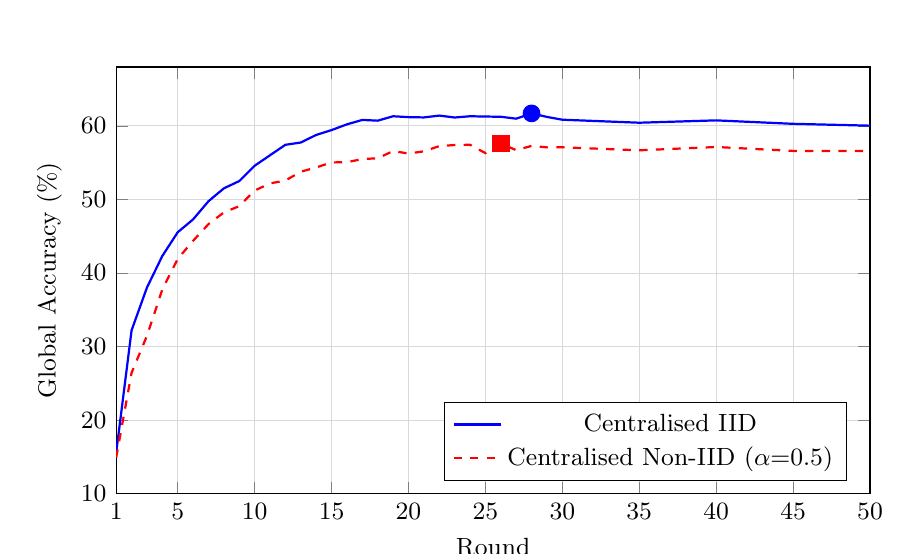
\begin{tikzpicture}
\begin{axis}[
  width=0.92\textwidth,
  height=7cm,
  xlabel={Round},
  ylabel={Global Accuracy (\%)},
  xmin=1, xmax=50,
  ymin=10, ymax=68,
  xtick={1,5,10,15,20,25,30,35,40,45,50},
  ytick={10,20,30,40,50,60,70},
  grid=both,
  grid style={line width=0.3pt, draw=gray!30},
  legend pos=south east,
  legend style={font=\small},
  tick label style={font=\small},
  label style={font=\small},
]
% Centralised IID
\addplot[color=blue, thick, mark=none] coordinates {
  (1,15.55)(2,32.19)(3,38.01)(4,42.31)(5,45.53)
  (6,47.28)(7,49.75)(8,51.50)(9,52.49)(10,54.57)
  (11,56.00)(12,57.42)(13,57.73)(14,58.76)(15,59.42)
  (16,60.20)(17,60.80)(18,60.70)(19,61.30)(20,61.18)
  (21,61.14)(22,61.39)(23,61.13)(24,61.30)(25,61.26)
  (26,61.23)(27,60.97)(28,61.69)(29,61.21)(30,60.83)
  (35,60.42)(40,60.74)(45,60.27)(50,60.02)
};
\addlegendentry{Centralised IID}
 
% Centralised Non-IID
\addplot[color=red, thick, dashed, mark=none] coordinates {
  (1,14.89)(2,26.42)(3,31.45)(4,37.76)(5,41.91)
  (6,44.37)(7,46.64)(8,48.23)(9,49.08)(10,51.20)
  (11,52.17)(12,52.56)(13,53.76)(14,54.34)(15,55.02)
  (16,55.06)(17,55.48)(18,55.59)(19,56.57)(20,56.23)
  (21,56.53)(22,57.24)(23,57.39)(24,57.42)(25,56.29)
  (26,57.60)(27,56.69)(28,57.27)(29,57.07)(30,57.08)
  (35,56.67)(40,57.12)(45,56.59)(50,56.58)
};
\addlegendentry{Centralised Non-IID ($\alpha{=}0.5$)}
 
% Peak markers
\addplot[color=blue, only marks, mark=*, mark size=3pt]
  coordinates {(28,61.69)};
\addplot[color=red, only marks, mark=square*, mark size=3pt]
  coordinates {(26,57.60)};
 
\end{axis}
\end{tikzpicture}
\caption{Global accuracy vs.\ round for Experiments 1 and 2 (Centralised
FedAvg). IID peaks at 61.69\% (Round 28); Non-IID peaks at 57.60\%
(Round 26). The gap stabilises at 3.4--5.1~pp from Round 12 onward.
Filled markers indicate peak accuracy points.}
\label{fig:centralised-convergence}
\end{figure}

Both experiments ran for approximately 22 minutes and transferred an identical
171,726--171,734 KB of data over 50 rounds. The data distribution has no impact
on communication cost in centralised FedAvg, since model size is fixed regardless
of local class distribution.

A structural observation from both experiments: every client's upload phase
blocks until all 7 clients have connected, and every download phase blocks until
the server broadcasts. During the 5-second inter-round wait, all 7 clients log
a failed connection attempt before successfully reconnecting. This synchronous
server dependency is the foundation of the SPOF risk demonstrated in
Experiment 5-B.

% ============================================================
\section{Decentralised Gossip FL: Experiments 3 and 4}
\label{sec:decentralised-results}
% ============================================================

\subsection{IID Results (Experiment 3)}

Under IID conditions, decentralised ring gossip converges to an average final
accuracy of \textbf{55.98\%} across 8 nodes (range: 55.37--56.79\%). All 8
nodes self-coordinated without any central server and completed 50/50 rounds.
No orchestration service or shared coordinator was involved.

The gossip blend provides a consistent +2 to +4 pp boost over each node's local
training accuracy per round. The spread in final accuracy across nodes is only
\textbf{1.42 pp} - approaching but not reaching the perfect uniformity
guaranteed by centralised FedAvg, where all clients receive the same
server-broadcast model each round.

Occasional negative blend events were observed - rounds where blending with
two neighbours briefly decreased accuracy (Round 3: $-$2.99 pp). These are
short-lived and the model recovers within 1--2 rounds. They occur when
neighbours' models are weakly trained early in the experiment and carry noise
rather than complementary knowledge. This higher round-to-round variance
compared to FedAvg is an inherent characteristic of averaging within a
small 2-neighbour neighbourhood.

\begin{figure}[H]
\centering

\includegraphics[width=0.95\textwidth]{Decentralized_IID}
\caption{Decentralised gossip - IID experiment, Round 3. Each node pushes
its model to both ring neighbours and blends three models (own + left + right).}
\label{fig:decentralised-iid-early}
\end{figure}

\subsection{Non-IID Results (Experiment 4)}

Under Non-IID conditions, average final accuracy drops to \textbf{49.49\%}
(range: 48.00--51.33\%) - a reduction of \textbf{6.49 pp} from the IID case.
This degradation is substantially larger than the 3.44 pp IID-to-Non-IID gap
observed in centralised FedAvg.

The reason is the smaller aggregation pool. In each round, a gossip node blends
only with its 2 immediate ring neighbours. If those neighbours carry correlated
class imbalances - as is likely under Non-IID when nearby ring positions share
similar data characteristics - the blend offers limited complementary knowledge.
FedAvg, by contrast, aggregates all 7 clients every round and sees the full
diversity of class distributions regardless of data heterogeneity.

The node accuracy spread under Non-IID is \textbf{3.33 pp} at Round 50 -
more than double the 1.42 pp spread under IID. Unlike centralised FL where all
clients always hold the same model, gossip nodes develop slightly different models
that reflect their local neighbourhood. Under Non-IID, this divergence is
amplified. This is not a bug but an inherent architectural property: gossip-based
FL does not guarantee model uniformity across nodes.

Despite this, the gossip blend remains valuable. Per-round blending boosts each
node's accuracy by +7 to +12 pp over its local model under Non-IID - 3 to 5
times the boost observed under IID. The local model alone is simply too
specialised to reach acceptable accuracy; neighbourhood knowledge is essential.

\begin{figure}[H]
\centering

\includegraphics[width=0.95\textwidth]{Decentralized_NonIID}
\caption{Decentralised gossip - Non-IID experiment, Round 8. Nodes exhibit
variable synchronisation delays due to differences in local training speed
under heterogeneous data.}
\label{fig:decentralised-noniid-early}
\end{figure}

Table~\ref{tab:decentralised-nodes} shows per-node final accuracy for both
decentralised experiments.

\begin{table}[H]
\centering
\begin{tabular}{lcc}
\toprule
\textbf{Node} & \textbf{IID Final Acc} & \textbf{Non-IID Final Acc} \\
\midrule
Node 0 & 56.56\% & 48.93\% \\
Node 1 & 55.89\% & 51.33\% \\
Node 2 & 55.71\% & 50.11\% \\
Node 3 & 56.34\% & 48.49\% \\
Node 4 & 55.80\% & 49.85\% \\
Node 5 & 55.64\% & 48.00\% \\
Node 6 & 55.37\% & 49.60\% \\
Node 7 & 56.79\% & 50.56\% \\
\midrule
\textbf{Average} & \textbf{55.98\%} & \textbf{49.49\%} \\
\textbf{Spread}  & \textbf{1.42 pp} & \textbf{3.33 pp} \\
\bottomrule
\end{tabular}
\vspace{0.5cm}
\caption{Per-node final accuracy - Decentralised Gossip (Round 50)}
\label{tab:decentralised-nodes}
\end{table}

Figure~\ref{fig:decentralised-convergence} plots the post-blend
accuracy per round for Node~0 (representative) in both decentralised
experiments. Node~0 is representative of the network average -
its final accuracy (56.17\% IID, 49.16\% Non-IID) is close to the
8-node averages (55.98\% and 49.49\% respectively).
 
\begin{figure}[H]
\centering
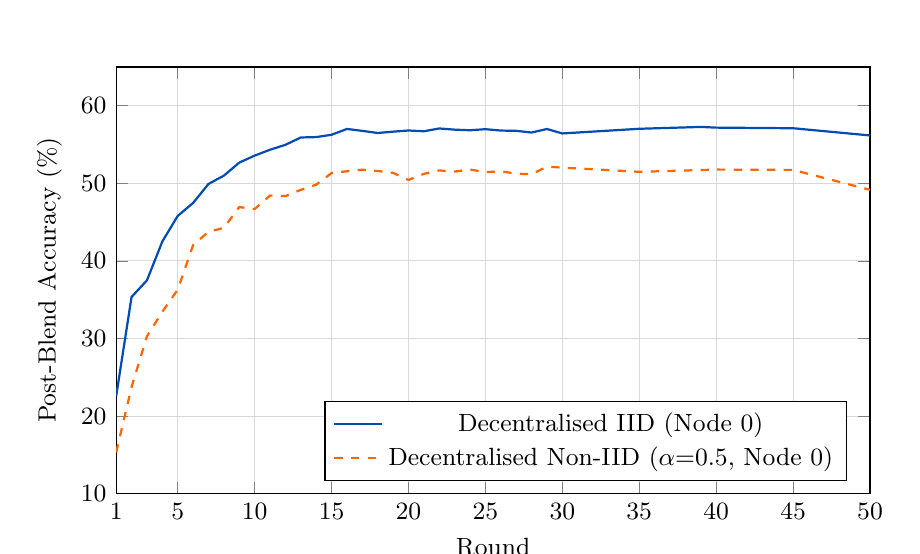
\begin{tikzpicture}
\begin{axis}[
  width=0.92\textwidth,
  height=7cm,
  xlabel={Round},
  ylabel={Post-Blend Accuracy (\%)},
  xmin=1, xmax=50,
  ymin=10, ymax=65,
  xtick={1,5,10,15,20,25,30,35,40,45,50},
  ytick={10,20,30,40,50,60,70},
  grid=both,
  grid style={line width=0.3pt, draw=gray!30},
  legend pos=south east,
  legend style={font=\small},
  tick label style={font=\small},
  label style={font=\small},
]
% Decentralised IID (Node 0 post-blend)
\addplot[color=blue!70!green, thick, mark=none] coordinates {
  (1,22.57)(2,35.35)(3,37.49)(4,42.50)(5,45.80)
  (6,47.47)(7,49.92)(8,50.99)(9,52.67)(10,53.57)
  (11,54.33)(12,54.96)(13,55.91)(14,55.96)(15,56.26)
  (16,57.01)(17,56.76)(18,56.49)(19,56.66)(20,56.81)
  (21,56.71)(22,57.07)(23,56.92)(24,56.84)(25,56.98)
  (26,56.80)(27,56.77)(28,56.55)(29,57.00)(30,56.43)
  (35,57.03)(39,57.27)(40,57.18)(45,57.10)(50,56.17)
};
\addlegendentry{Decentralised IID (Node 0)}
 
% Decentralised Non-IID (Node 0 post-blend)
\addplot[color=orange!80!red, thick, dashed, mark=none] coordinates {
  (1,15.31)(2,23.75)(3,30.29)(4,33.44)(5,36.29)
  (6,42.04)(7,43.76)(8,44.26)(9,46.94)(10,46.68)
  (11,48.42)(12,48.35)(13,49.16)(14,49.83)(15,51.32)
  (16,51.56)(17,51.76)(18,51.59)(19,51.35)(20,50.43)
  (21,51.22)(22,51.66)(23,51.51)(24,51.78)(25,51.44)
  (26,51.55)(27,51.24)(28,51.18)(29,52.14)(30,52.03)
  (35,51.48)(40,51.77)(45,51.73)(50,49.16)
};
\addlegendentry{Decentralised Non-IID ($\alpha{=}0.5$, Node 0)}
 
\end{axis}
\end{tikzpicture}
\caption{Post-blend accuracy vs.\ round for Experiments 3 and 4
(Decentralised Gossip, Node~0). IID converges to $\sim$57\% and
holds steadily from Round~15. Non-IID plateaus at $\sim$51--52\%
from Round~15, never crossing 53\% sustainably. The gap between
IID and Non-IID ($\sim$7~pp) is wider than in centralised FL
($\sim$3.5~pp), confirming gossip's greater sensitivity to data
heterogeneity.}
\label{fig:decentralised-convergence}
\end{figure}

The model exchange step --- the actual bytes-on-wire transfer --- completes
in under five seconds per round in both architectures. Under IID conditions,
each gossip node completes its two-neighbour exchange in one to two seconds.
In the centralised setup, the server broadcast and the subsequent client
upload together take four to seven seconds per round. Neither architecture
is communication-bound: local training dominates round duration in both cases
(approximately five local epochs of CNN training), and communication adds a
comparatively small overhead on top.

Under Non-IID data conditions, the gossip exchange time becomes more variable
across nodes. Because Dirichlet partitioning assigns different class mixes to
each node, some nodes complete local training systematically faster than their
ring neighbours. A node that finishes training earlier will find its neighbours
not yet listening, triggering retry delays and pushing its exchange time toward
three to four seconds per round. This is a direct system-level consequence of
data heterogeneity --- one that operates independently of the accuracy
degradation already discussed.

The more fundamental distinction between the two architectures is not
communication latency but \emph{dependency scope}. In centralised FL, every
round is gated on all seven clients responding to the server; one slow or
unreachable client stalls the entire round. In gossip FL, each node is gated
only on its two immediate neighbours --- the remaining six nodes proceed
independently. In production-scale deployments, where the number of
participants can reach hundreds or thousands, this distinction becomes
decisive: centralised FL must wait for the slowest of all participants each
round, while gossip's wait is bounded by two neighbours regardless of network
size.

% ============================================================
\section{Architecture Comparison: Experiments 1--4}
\label{sec:architecture-comparison}
% ============================================================

Table~\ref{tab:arch-comparison} directly compares the key results from
Experiments 1--4.

\begin{table}[H]
\centering
\small
\begin{tabular}{lp{2cm}p{2.2cm}p{1.9cm}p{2.2cm}}
\toprule
\textbf{Metric}
  & \textbf{Centralised IID}
  & \textbf{Centralised Non-IID}
  & \textbf{Gossip IID}
  & \textbf{Gossip Non-IID} \\
\midrule
Peak accuracy    & 61.69\% & 57.60\% & 57.48\% & 53.44\% \\
Final accuracy   & 60.02\% & 56.58\% & 55.98\% & 49.49\% \\
Rounds to 50\%   & R8      & R10     & R8      & R15     \\
Accuracy spread  & 0 pp    & 0 pp    & 1.42 pp & 3.33 pp \\
Avg round duration & $\sim$16s & $\sim$16s & $\sim$24s & $\sim$24s \\
Comm. scope      & All 7 clients & All 7 clients & 2 neighbours & 2 neighbours \\
Nodes completed  & 7/7     & 7/7     & 8/8     & 8/8     \\
\bottomrule
\end{tabular}
\vspace{0.5cm}
\caption{Architecture comparison - normal operation results}
\label{tab:arch-comparison}
\end{table}

The accuracy gap between centralised FedAvg and decentralised gossip is
\textbf{4.21 pp under IID} and \textbf{7.09 pp under Non-IID} (comparing
final accuracy). The gap is larger under Non-IID because gossip's small
neighbourhood is less effective than FedAvg's full global aggregation at
overcoming class imbalance. This is the quantified accuracy cost of
eliminating the central server.

The round duration difference --- approximately 16~seconds for centralised FL
versus approximately 24~seconds for gossip --- is driven by local training
time, not by the communication protocol. Both architectures complete their
model exchange in under ten seconds per round; the extra eight seconds in
gossip come from five local training epochs on the same hardware. Neither
architecture is communication-bound.

The structurally important difference is \emph{dependency scope}, not
communication latency. In centralised FL, every round is gated on all seven
clients simultaneously: one unresponsive client delays the entire system, and
one failed server halts every client permanently. In gossip FL, each node's
round is gated only on its two ring neighbours; delays are absorbed locally
and do not propagate system-wide. This property scales favourably: in a
real-world deployment with hundreds of participants, centralised FL's wait
grows with the number of clients, while gossip's wait remains bounded by two
neighbours regardless of network size.

% ============================================================
\section{Fault Injection: Experiments 5-A and 5-B}
\label{sec:fault-results}
% ============================================================

Both fault experiments used Non-IID data and identical model/hardware setups.
In Experiment 5-A, Node 3 was killed after completing Round 10. In Experiment
5-B, the server was killed after completing Round 9's broadcast. The outcome
in each case was fundamentally different.

\subsection{Experiment 5-B: SPOF in Centralised FL}

The server was terminated after broadcasting the Round~9 aggregated model to all
7 clients. All clients completed their Round~10 local training and began
attempting to upload to the now-unavailable server.

Each client retried the upload at regular intervals for up to 300 seconds. After
exhausting all retry attempts, all 7 clients simultaneously logged a critical
connectivity failure and ceased operation. The system halted permanently at 9/50
rounds with a final accuracy of \textbf{49.07\%}. No client could continue,
recover, or route around the failure.

The potential accuracy the system would have reached with a healthy server -
based on Experiment 2 - was 57.60\%. The SPOF caused a permanent accuracy
loss of approximately \textbf{8.5 pp} and 41 rounds of training time with no
recovery path.

\begin{figure}[H]
\centering

\includegraphics[width=0.95\textwidth]{Centralized_SPOF}
\caption{Centralised SPOF experiment - early training (Round~5), showing
normal operation prior to server termination. All 7 clients are connected
and training progresses as expected.}
\label{fig:centralised-spof-normal}
\end{figure}

\begin{figure}[H]
\centering

\includegraphics[width=0.95\textwidth]{Centralized_SPOF_5}
\caption{Centralised SPOF experiment after server termination. All client
terminals report repeated connection failures; no client is able to
proceed without the server.}
\label{fig:centralised-spof-infra}
\end{figure}

\subsection{Experiment 5-A: Fault Tolerance in Decentralised FL}

\begin{figure}[H]
\centering
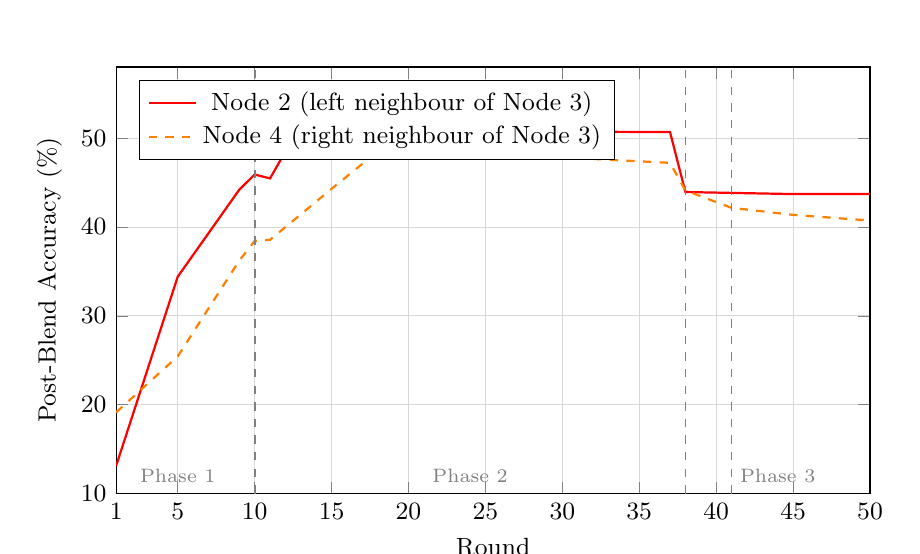
\begin{tikzpicture}
\begin{axis}[
  width=0.92\textwidth,
  height=7cm,
  xlabel={Round},
  ylabel={Post-Blend Accuracy (\%)},
  xmin=1, xmax=50,
  ymin=10, ymax=58,
  xtick={1,5,10,15,20,25,30,35,40,45,50},
  ytick={10,20,30,40,50,60},
  grid=both,
  grid style={line width=0.3pt, draw=gray!30},
  legend pos=north west,
  legend style={font=\small},
  tick label style={font=\small},
  label style={font=\small},
]
% Node 2 accuracy (3 phases)
\addplot[color=red, thick, mark=none] coordinates {
  (1,13.14)(5,34.40)(9,44.19)(10,45.90)
  (11,45.46)(13,51.50)(20,51.11)(30,50.72)(37,50.68)
  (38,43.93)(45,43.70)(50,43.70)
};
\addlegendentry{Node 2 (left neighbour of Node 3)}
% Node 4 accuracy
\addplot[color=orange, thick, dashed, mark=none] coordinates {
  (1,19.15)(5,25.44)(9,36.21)(10,38.42)
  (11,38.55)(15,44.29)(19,49.92)(30,47.83)(37,47.21)
  (38,44.10)(41,42.15)(45,41.36)(50,40.72)
};
\addlegendentry{Node 4 (right neighbour of Node 3)}
% Phase boundary lines
\draw[dashed, gray, thick] (axis cs:10,10) -- (axis cs:10,58)
  node[above, font=\scriptsize, text=gray] {Node 3 fails};
\draw[dashed, gray] (axis cs:38,10) -- (axis cs:38,58)
  node[above, font=\scriptsize, text=gray] {N2 isolated};
\draw[dashed, gray] (axis cs:41,10) -- (axis cs:41,58)
  node[above, font=\scriptsize, text=gray] {N4 isolated};
% Phase labels
\node[font=\scriptsize, text=gray] at (axis cs:5,12) {Phase 1};
\node[font=\scriptsize, text=gray] at (axis cs:24,12) {Phase 2};
\node[font=\scriptsize, text=gray] at (axis cs:44,12) {Phase 3};
\end{axis}
\end{tikzpicture}
\caption{Per-round accuracy of Nodes~2 and~4 (direct neighbours of failed
Node~3) in Experiment~5-A. Phase~1 (R1--10): normal operation with both
neighbours. Phase~2 (R11--37/41): one surviving neighbour; accuracy holds
but round time inflates. Phase~3 (R38/41--50): complete isolation; accuracy
frozen at local training output ($\sim$43--44\%).}
\label{fig:fault-node-accuracy}
\end{figure}

Node~3 completed its Round~10 blend and was then terminated. Its direct ring
neighbours - Node~2 on the left and Node~4 on the right - detected the
absence via a push timeout, approximately 90 seconds after the exit. Both
logged a push failure for Node~3 and continued training with their remaining
neighbour.

All 7 remaining nodes completed 50/50 rounds. The system never halted.

\begin{figure}[H]
\centering

\includegraphics[width=0.95\textwidth]{Decentralized_FaultTolerance}
\caption{Decentralised fault tolerance (Experiment~5-A) - Nodes~2 and~4
detecting the absence of Node~3. Both nodes log the push failure and
continue training with their remaining ring neighbour.}
\label{fig:decentralised-fault-early}
\end{figure}

\begin{figure}[H]
\centering

\includegraphics[width=0.95\textwidth]{Decentralized_FaultTolerance_5}
\caption{Decentralised fault tolerance - Round 46. All surviving nodes
continue making progress, with Nodes 2 and 4 showing reduced accuracy due
to limited blending after Node 3's exit.}
\label{fig:decentralised-fault-late}
\end{figure}

\subsection{The Cascading Timing-Drift Effect}

An unexpected finding emerged from the fault experiment. Because the synchronous
gossip protocol requires each node to wait for both neighbours to push their
models, Node 3's absence caused Nodes 2 and 4 to wait for the full 90-second
push retry timeout before proceeding. This inflated their round duration from
approximately 37 seconds to approximately 130 seconds per round.

This timing inflation had a cascading effect. When Nodes 2 and 4 consistently
ran 90 seconds late per round, their surviving neighbours - Node 1 (adjacent
to Node 2) and Node 5 (adjacent to Node 4) - began timing out on their push
attempts to Nodes 2 and 4 as well. By Round 38, Node 2 had lost connectivity
to both its remaining neighbours and began training in complete isolation. Node
4 followed at Round 41.

The timing disruption propagated outward from the failed node with measurable
distance decay:

\begin{table}[H]
\centering
\caption{Communication time inflation by ring distance from failed Node 3}
\label{tab:timing-drift}
\begin{tabular}{lcc}
\toprule
\textbf{Distance from Node 3} & \textbf{Avg comm time} & \textbf{Inflation} \\
\midrule
1 hop (Nodes 2, 4)    & $\sim$96--130s & +303\% \\
2 hops (Nodes 1, 5)   & $\sim$65s      & +172\% \\
3 hops (Nodes 0, 6)   & $\sim$51s      & +114\% \\
4 hops (Node 7)       & $\sim$49s      & +104\% \\
\bottomrule
\end{tabular}
\end{table}

\begin{figure}[H]
\centering
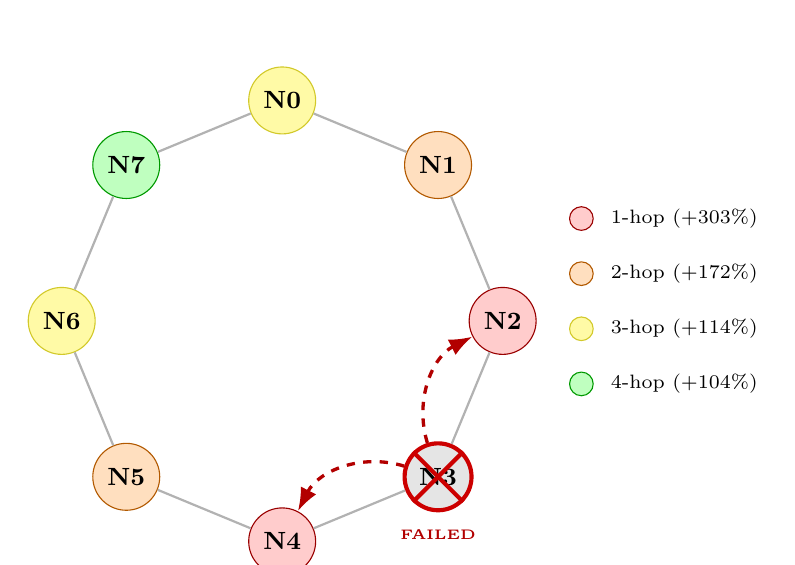
\begin{tikzpicture}[
  ringnode/.style={circle, draw, minimum size=0.85cm, font=\small\bfseries, inner sep=0pt},
  failed/.style={ringnode, fill=gray!20, draw=red!80!black, line width=1.5pt},
  hop1/.style={ringnode, fill=red!20, draw=red!60!black},
  hop2/.style={ringnode, fill=orange!25, draw=orange!70!black},
  hop3/.style={ringnode, fill=yellow!35, draw=yellow!80!black},
  hop4/.style={ringnode, fill=green!25, draw=green!60!black},
  ringedge/.style={thick, gray!60},
  cascarrow/.style={-{Latex}, dashed, red!70!black, line width=1.2pt}
]
  \def\R{2.8}
  \node[hop3]   (n0) at (90:\R)   {N0};
  \node[hop2]   (n1) at (45:\R)   {N1};
  \node[hop1]   (n2) at (0:\R)    {N2};
  \node[failed] (n3) at (-45:\R)  {N3};
  \node[hop1]   (n4) at (-90:\R)  {N4};
  \node[hop2]   (n5) at (-135:\R) {N5};
  \node[hop3]   (n6) at (180:\R)  {N6};
  \node[hop4]   (n7) at (135:\R)  {N7};
  \draw[ringedge] (n0)--(n1)--(n2)--(n3)--(n4)--(n5)--(n6)--(n7)--(n0);
  \draw[cascarrow] (n3) to[bend left=40] (n2);
  \draw[cascarrow] (n3) to[bend right=40] (n4);
  \draw[red!80!black, line width=1.5pt] (n3.north west)--(n3.south east);
  \draw[red!80!black, line width=1.5pt] (n3.north east)--(n3.south west);
  \node[font=\tiny\bfseries, text=red!70!black, below=3pt of n3] {FAILED};
  % Legend
  \node[circle, draw=red!60!black,   fill=red!20,    minimum size=0.3cm, inner sep=0pt] at (3.8, 1.3) {};
  \node[anchor=west, font=\scriptsize] at (4.05, 1.3) {1-hop (+303\%)};
  \node[circle, draw=orange!70!black, fill=orange!25, minimum size=0.3cm, inner sep=0pt] at (3.8, 0.6) {};
  \node[anchor=west, font=\scriptsize] at (4.05, 0.6) {2-hop (+172\%)};
  \node[circle, draw=yellow!80!black, fill=yellow!35, minimum size=0.3cm, inner sep=0pt] at (3.8,-0.1) {};
  \node[anchor=west, font=\scriptsize] at (4.05,-0.1) {3-hop (+114\%)};
  \node[circle, draw=green!60!black,  fill=green!25,  minimum size=0.3cm, inner sep=0pt] at (3.8,-0.8) {};
  \node[anchor=west, font=\scriptsize] at (4.05,-0.8) {4-hop (+104\%)};
\end{tikzpicture}
\caption{Cascading timing-drift propagation from failed Node~3. Colour encodes
ring distance from the failure. Dashed red arrows indicate the cascade direction
that caused secondary isolation of Nodes~2 and~4.}
\label{fig:cascade-ring}
\end{figure}

The accuracy impact was localised to the two direct neighbours. Nodes 2 and 4
finished with final accuracies of 43.70\% and 40.72\% respectively - drops
of 7.63 pp and 9.13 pp compared to their baselines in Experiment 4. All other
5 surviving nodes finished within $\pm$2 pp of their normal Non-IID baselines.

This cascading isolation behaviour - where a single failed node eventually
causes its direct neighbours to lose \textit{all} connectivity through secondary
timing effects - was not predicted by theoretical gossip FL models. It is a
real-world TCP timeout behaviour that only becomes visible on actual distributed
infrastructure.

\subsection{Direct Comparison of Fault Outcomes}

Table~\ref{tab:fault-comparison} summarises the direct comparison between
Experiments 5-A and 5-B.

\begin{table}[H]
\centering
\small
\begin{tabular}{lp{4.5cm}p{4.5cm}}
\toprule
\textbf{Metric}
  & \textbf{Experiment~5-A (Decentralised)}
  & \textbf{Experiment~5-B (Centralised)} \\
\midrule
Failed component   & Node~3 (1 of 8 ring nodes)     & Server (sole coordinator) \\
Nodes continuing   & \textbf{7/8 - all 50 rounds}  & \textbf{0/7 - halted at R9} \\
System halt        & \textbf{No}                     & \textbf{Yes, permanent} \\
Final accuracy     & 48.68\% avg (7 surviving nodes) & 49.07\% (frozen at R9) \\
Accuracy lost      & 7.6--9.1~pp (2 direct neighbours) & $\sim$8.5~pp (all 7 nodes) \\
Failure detection  & $\sim$90~s (push timeout)       & $\sim$4~min (retry exhaustion) \\
Recovery possible  & Yes - partial                  & No \\
\bottomrule
\end{tabular}
\vspace{0.5cm}
\caption{Fault experiment outcomes: decentralised vs.\ centralised}
\label{tab:fault-comparison}
\end{table}

The comparison is stark. In centralised FL, 1 server failure equals 7 client
failures and 100\% system halt. In decentralised ring gossip, 1 node failure
equals 2 degraded neighbours and 5 unaffected nodes, with 0\% system halt.
The 2 directly affected nodes lost accuracy but never stopped training. In
centralised FL, all 7 clients lost 82\% of their planned training budget
instantly and permanently.

% ============================================================
\section{Graph Topology Comparison: Experiments 6-A, 6-B, and 6-C}
\label{sec:topology-results}
% ============================================================

A second pair of decentralised experiments repeated the IID and Non-IID
evaluation with all other variables held fixed, replacing only the ring graph
(degree~2, diameter~4) with a fully-connected graph (degree~7, diameter~1).
In the fully-connected topology, every node communicates directly with all
other nodes each round. The blend pool expands from three models (self plus
two ring neighbours) to eight models spanning the entire network -- equivalent
to running a global average without a central server.

\subsection{IID Results: Fully Connected vs Ring}

Under IID data, fully-connected gossip reached a final accuracy of 61.17\%,
compared to 55.98\% for ring gossip -- a gain of \textbf{5.19~pp}. The best
accuracy achieved across all rounds was 61.74\% at Round~25, versus 57.48\% at
Round~21 for the ring. The ring never exceeded 57.5\% across all 50 rounds;
the fully-connected topology crossed 60\% accuracy by Round~19 and remained
above it until the end.

A structurally notable result is that all eight fully-connected nodes converged
to exactly the same accuracy every round -- a final variance of \textbf{0.00~pp}
across all nodes. The ring, by contrast, retained a final accuracy spread of
55.37--56.79\% (range 1.42~pp). This is a direct consequence of the
fully-connected graph's diameter of 1: every node receives every other node's
model at every round, which is mathematically equivalent to computing a global
FedAvg average at each step.

\subsection{Non-IID Results: Fully Connected vs Ring}

Under Non-IID data, the fully-connected topology achieved a final accuracy of
57.99\%, compared to 49.49\% for the ring -- a gain of \textbf{8.50~pp}. The
accuracy advantage is larger under Non-IID than under IID (8.50~pp
vs 5.19~pp), which directly validates the theoretical claim of \citet{tang2018d2}:
increased connectivity specifically counteracts the accuracy penalty of data
heterogeneity. A node in a ring receives only two models per round, both from
nearby nodes that may hold similarly skewed class distributions. A node in a
fully-connected graph receives all seven peers' models, which collectively span
the full class distribution across the network, effectively cancelling local
skew at each blend step.

The most striking single finding across all experiments is the following
cross-condition comparison: \textbf{FC Non-IID (57.99\%) outperforms Ring IID
(55.98\%)}. Full connectivity with heterogeneous data outperforms sparse connectivity
with uniform data. This means that for networks where Non-IID conditions are
unavoidable, switching from ring to fully-connected topology is sufficient to
recover more accuracy than the heterogeneity cost -- a result with direct
practical implications for deployment topology selection.

As in the IID case, all eight nodes converged to exactly the same accuracy
under fully-connected Non-IID conditions (zero inter-node variance), compared
to a 3.33~pp spread across ring nodes (48.00--51.33\%).

\subsection{Communication Analysis}

\begin{table}[H]
\centering
\begin{tabular}{lcccc}
\toprule
\textbf{Metric} & \textbf{Ring IID} & \textbf{FC IID} & \textbf{Ring Non-IID} & \textbf{FC Non-IID} \\
\midrule
Final accuracy (avg)      & 55.98\%  & \textbf{61.17\%} & 49.49\%  & \textbf{57.99\%} \\
Best accuracy (avg)       & 57.06\%  & \textbf{61.74\%} & 51.67\%  & \textbf{58.81\%} \\
Accuracy gain (FC vs Ring)& ---      & +5.19~pp         & ---      & +8.50~pp \\
Node accuracy variance    & $\pm$0.71\% & \textbf{0.00\%} & $\pm$1.57\% & \textbf{0.00\%} \\
Avg comm time / round     & 24.6~s   & \textbf{3.4~s}  & 24.2~s   & \textbf{1.9~s} \\
Avg round duration        & 36.5~s   & \textbf{15.4~s} & 35.1~s   & \textbf{14.1~s} \\
Total comm volume / node  & 47.9~MB  & 167.7~MB        & 47.9~MB  & 167.7~MB \\
\bottomrule
\end{tabular}
\vspace{0.5cm}
\caption{Ring vs fully-connected topology: accuracy and communication comparison}
\label{tab:topology-comparison}
\end{table}

An unexpected result emerges from the communication timing data. Despite
transmitting 3.5$\times$ more data per round (167.7~MB vs 47.9~MB per node
over 50 rounds), the fully-connected topology completed each round
\textbf{2.4$\times$ faster} (15.4~s vs 36.5~s per round). The apparent
paradox is explained by the synchronisation structure of each topology.

In synchronous ring gossip, each node must push to and receive from two
neighbours. Because all nodes are executing simultaneously, the push-receive
cycle creates a ring-wide sequential dependency: each node's push success
depends on the neighbouring node being ready to receive, which in turn
depends on that node having received from its other neighbour. This chained
dependency produces an average per-round communication time of $\sim$24~s --
substantially longer than the time required to physically transfer
the model over the VPC.

In the fully-connected topology, each node pushes to all peers simultaneously
using concurrent connections. The per-round wall-clock communication time is
bounded by only the \emph{single slowest connection}, not a chain of sequential
dependencies. All pushes and receives overlap, collapsing the effective
communication time to $\sim$3~s. The correct interpretation is therefore: the
fully-connected topology's higher bandwidth cost is more than offset by the
elimination of ring gossip's synchronisation bottleneck through parallelism.

\subsection{Fault Propagation Under Full Connectivity}
\label{sec:fc-fault}

An attempt was made to replicate the node-exit fault scenario from the ring
fault experiment under the fully-connected topology, to compare fault impact
structure across the two graph designs. The attempt revealed a structural
impracticality specific to the fully-connected topology under persistent node
failure, which is itself a meaningful result.

In the ring fault experiment, the failure of one node caused exactly two nodes
-- its direct ring neighbours -- to experience a TCP push timeout on every
subsequent round. The remaining nodes were entirely unaffected and completed
all 50 rounds at normal speed. The fault impact was \emph{localised} to the
edges directly connected to the failed node.

In the fully-connected topology, the equivalent single-node exit caused all
surviving nodes to experience the push timeout simultaneously, because every
node maintains an edge to every other node. Each surviving node also received
fewer peer models than expected per round, causing receive-side timeouts to
fire across all surviving nodes at once. The per-round communication time
for every surviving node inflated dramatically from normal fully-connected
levels, dominated by connection timeout expiry rather than actual training
or data transfer. Sustained over the remaining training rounds, this produced
a prolonged period of timeout-dominated execution across the entire surviving
network simultaneously.

The experiment could not be completed stably under these conditions. The
cumulative effect of all surviving nodes running well below their normal round
speed caused synchronisation drift and resource accumulation that destabilised
several instances before training completed.

This outcome confirms a fundamental structural property. In a graph of degree
$d$, one node failure generates $d$ simultaneous timeouts per round. For
the ring ($d = 2$), this is 2 timeouts -- affecting only the two direct
neighbours. For the fully-connected graph ($d = N-1$), this is $N-1$
timeouts -- one per surviving node. The fault isolation provided by the ring
is a direct consequence of its sparsity: the property that limits convergence
speed under normal operation provides natural containment under fault
conditions. Table~\ref{tab:fault-topology} summarises the structural
contrast between the two topologies.

\begin{table}[H]
\centering
\begin{tabular}{lcc}
\toprule
\textbf{Property} & \textbf{Ring Topology} & \textbf{Fully Connected} \\
\midrule
Nodes detecting fault          & 2 of 7              & 7 of 7 \\
TCP timeouts per round         & 2                   & 7 \\
Fault impact                   & Localised           & Global \\
Nodes unaffected               & 5 of 7              & 0 of 7 \\
Round slowdown (affected)      & $\sim$3.5$\times$   & $\sim$8$\times$ \\
System stable to Round 50      & Yes                 & No (experiment terminated) \\
Graph property responsible     & Low degree (2)      & High degree (7) \\
\bottomrule
\end{tabular}
\vspace{0.5cm}
\caption{Fault impact structure: ring vs fully-connected topology}
\label{tab:fault-topology}
\end{table}

This topology comparison therefore establishes a fundamental structural finding:
the ring's sparsity, which is a liability for accuracy and convergence speed
under normal operation, is an asset for fault containment. The fully-connected
topology's density, which benefits convergence under normal operation, becomes
a liability under persistent failure. This trade-off is analytically derived
from graph degree and does not require a completed run to establish -- the
O($N-1$) timeout cascade is a structural property of the graph, not a
contingent empirical finding.

% ============================================================
\section{Threats to Validity}
\label{sec:threats}
% ============================================================

\subsection*{Internal Validity}

The fault experiments (5-A and 5-B) compare different architectures by design.
The failure outcome is therefore attributed to the structural difference in
topology - the presence or absence of a central coordinator - rather than
to any confounding variable, since hardware, dataset, model, and data
distribution were held identical across both experiments.

The 90-second TCP push retry timeout governs when cascading isolation first
appears in Experiment~5-A. This is a deliberate protocol configuration, not an
uncontrolled variable. Its value is explicitly reported (Section~\ref{sec:fault-results})
so that replication studies can reproduce or vary the timeout to test its effect
on cascade onset and severity.

\subsection*{External Validity}

All 8 EC2 instances were homogeneous \texttt{t3.micro} nodes with identical
hardware and network conditions. Straggler effects arising from heterogeneous
hardware - a common real-world condition where some devices are significantly
slower than others - were not studied. The reported round times and cascade
thresholds may differ in deployments with hardware diversity.

The ring diameter at 8 nodes is 4 hops. Knowledge propagation speed and fault
cascade behaviour are both functions of ring size. At 64 nodes the diameter
grows to 32 hops, and the timing-drift cascade may resolve before reaching all
nodes, or may propagate further than observed here. Scaling behaviour was not
studied and constitutes the most direct extension of this work.

\subsection*{Construct Validity}

Accuracy is measured as post-blend accuracy evaluated on the full 10,000-image
CIFAR-10 test set after each round's blend step, capturing the effective model
quality a node would deploy rather than raw local training accuracy.
Per-round communication time includes the training wait for neighbours to
complete their local epoch, making it a round wall-time measure that captures
both computation and communication latency rather than pure network transfer time.

\subsection*{Conclusion Validity}

Experiments 1--4 were repeated across multiple independent sessions under
identical configuration. Results were consistent within 0.33~pp across sessions,
confirming that the reported accuracy values are stable and not artefacts of a
single run. The fault experiments (5-A and 5-B) were each executed as a single
run by design: fault injection is a one-time deterministic intervention, and
repeating it under identical conditions - fixed seed, same component terminated
at the same round - would produce identical outcomes.

\chapter{Conclusion}

The experiments confirm that decentralised gossip FL achieves accuracy
comparable to centralised FedAvg at a quantified cost. Under IID conditions,
ring gossip reached a final accuracy of 55.98\% versus 60.02\% for FedAvg --
a gap of 4.04~pp -- with both architectures crossing 50\% accuracy at the same
training round, confirming similar early-phase convergence behaviour. This gap
widens under Non-IID data: ring gossip's accuracy dropped by 6.49~pp from its
IID baseline to 49.49\%, compared to a 3.44~pp drop for FedAvg to 56.58\%.
The asymmetry is structural. Each gossip node blends only with its two immediate
ring neighbours per round, making it more vulnerable to correlated class
imbalances within its local neighbourhood. FedAvg, aggregating all clients every
round, is inherently more robust to data heterogeneity. The accuracy cost of
removing the central server is therefore real and measurable, and it grows
meaningfully under the non-uniform data conditions typical of real-world
deployments.

The fault injection experiments reveal the fundamental structural difference
between the two architectures. In centralised FL, a single server failure caused
all seven clients to exhaust their retry budgets and halt permanently, with no
recovery path and 41 rounds of planned training permanently lost at a frozen
accuracy of 49.07\%. In decentralised FL, the equivalent single-node failure
had no system-wide effect: all seven remaining nodes completed all 50 training
rounds without halting. The two direct ring neighbours of the failed node
experienced accuracy drops of 7.6--9.1~pp but continued training throughout;
the remaining five nodes finished within $\pm$2~pp of their normal baselines.
The contrast is unambiguous -- one server failure produces a complete and
permanent system halt, while one node failure in the decentralised setting is
absorbed locally. The decentralised architecture eliminates the Single Point
of Failure.

Real deployment on distributed infrastructure revealed a secondary effect not
predicted by existing gossip FL theory. When a node failed, its direct ring
neighbours accumulated a communication retry delay per round that substantially
inflated their round duration. This timing drift cascaded outward: the affected
neighbours eventually lost synchronisation with their own surviving neighbours,
causing complete isolation in later training rounds. The inflation decayed with
ring distance but remained measurable four hops from the failed node. This
emergent cascading behaviour -- where a single node failure causes secondary
isolation through accumulated timeout delays across the ring -- is not captured
by theoretical gossip models, which assume clean binary message delivery. It is
a real-world system property that only becomes observable on actual distributed
infrastructure.

Graph topology proved to be a decisive design parameter within the decentralised
setting. Replacing the ring with a fully-connected graph, with no other change to
the model, dataset, or protocol, produced accuracy gains of 5.19~pp under IID
and 8.50~pp under Non-IID. The larger Non-IID gain confirms that higher
connectivity counteracts data heterogeneity: the fully-connected blend pool
samples the full network class distribution each round, neutralising local skew
that persists across many rounds in the ring. The fully-connected topology also
eliminated inter-node accuracy variance entirely and completed each round
2.4$\times$ faster despite transmitting 3.5$\times$ more data, as concurrent
peer communication removes the ring's sequential synchronisation bottleneck.
Under fault conditions, however, the topology's advantage reverses: the ring
contains any single node failure to two direct neighbours, while the
fully-connected graph propagates the failure impact to all surviving nodes
simultaneously. This accuracy-versus-fault-isolation trade-off is a structural
consequence of graph degree and holds independently of the specific experimental
configuration.

\section{Summary of Work}

This thesis set out to answer a question that the federated learning literature
had left unanswered: what actually happens when a server or node fails during
training on real distributed infrastructure, and how much accuracy does a
decentralised architecture sacrifice to eliminate that risk?

To answer this, both a centralised FedAvg system and a decentralised synchronous
gossip FL system were built from scratch in Python and PyTorch, deployed on
8 real AWS EC2 instances, and evaluated across nine controlled experiments covering
IID and Non-IID data distributions, normal operation, live failure injection, and
a topology comparison between ring and fully-connected gossip graphs.
An earlier two-node pilot on VMware VMs confirmed the P2P communication
infrastructure and produced an unplanned server crash that directly motivated the
deliberate fault injection experiments.

\section{Key Findings}

\textbf{The accuracy cost of decentralisation is small and consistent.}
Decentralised gossip FL reached within 4.21 pp of centralised FedAvg under IID
conditions (55.98\% vs 60.02\% final accuracy) and within 7.09 pp under Non-IID
(49.49\% vs 56.58\%). Both architectures converged to 50\% accuracy within a
similar number of rounds under IID. The accuracy gap is real but modest, and
represents the measurable price of eliminating the central server entirely.

\textbf{Gossip FL is more sensitive to Non-IID data than FedAvg.}
The IID-to-Non-IID accuracy drop was 6.49 pp in the decentralised setting versus
3.44 pp in the centralised setting. This is because each gossip node blends with
only 2 immediate neighbours per round, making it vulnerable to correlated class
imbalances in its local neighbourhood. FedAvg aggregates all 7 clients every
round and sees the full diversity of class distributions, making it more robust
to data heterogeneity.

\textbf{The SPOF is real and total.}
When the server was terminated after Round~9, all 7 clients exhausted their
retry budgets and halted permanently. The system froze at 49.07\% accuracy
with 41 rounds of training permanently lost. No client could continue or
recover without a manual server restart.

\textbf{Communication dependency is local, not global.}
In centralised FL, every round stalls if any single client is unreachable
from the server. In gossip FL, each node is gated only on its two immediate
neighbours; all other nodes proceed independently. This difference in
dependency scope --- global versus local --- is why the two fault experiments
produce such structurally different outcomes from an identical triggering
event.

\textbf{Decentralised FL survives node failure.}
When a node was terminated mid-training, all remaining nodes completed all 50
rounds. The system never halted. The two direct neighbours saw accuracy drops
of 7.63 pp and 9.13 pp respectively, but continued training throughout.
All other nodes finished within $\pm$2 pp of their normal baselines.

\textbf{Graph topology is a decisive factor in decentralised FL performance.}
Switching from ring to fully-connected topology -- with no other change --
produced accuracy gains of 5.19~pp under IID and 8.50~pp under Non-IID.
The Non-IID gain being larger confirms that higher connectivity specifically
counteracts data heterogeneity: the fully-connected blend pool samples the
full network class distribution each round, neutralising local skew that
persists across many rounds in the ring. The most striking cross-condition
result is that \emph{FC Non-IID (57.99\%) outperforms Ring IID (55.98\%)}:
heterogeneous data under full connectivity produces better accuracy than
uniform data under a ring. Fully-connected gossip also eliminated all
inter-node accuracy variance (0.00~pp vs up to 3.33~pp), and completed
each round 2.4$\times$ faster despite transmitting 3.5$\times$ more data,
as parallel communication collapses the ring's chain-synchronisation overhead.

\textbf{Topology determines fault isolation scope.}
Under normal operation, the ring's low degree is a liability. Under fault
conditions, it becomes an asset. When one node failed in the ring topology,
only its two directly-connected neighbours experienced communication delays;
the remaining nodes were completely unaffected. The equivalent experiment under fully-connected topology
showed the opposite: all surviving nodes simultaneously experienced the failure
impact, because every node holds an edge to every other node. The fault impact
scales with graph degree -- localised to direct neighbours in sparse graphs
and global across the network in dense graphs. This structural contrast --
confirmed analytically and partially empirically -- establishes that ring and
fully-connected topologies represent a fundamental accuracy-versus-fault-isolation
trade-off, not a simple domination relationship.

\textbf{A previously undescribed cascading failure behaviour was discovered.}
When the node failed, the TCP push timeout at its direct neighbours substantially
inflated their round duration. This timing drift cascaded outward: the affected
neighbours eventually lost synchronisation with their own surviving neighbours
as well, becoming fully isolated in later training rounds. The timing inflation
decayed measurably with ring distance but was still detectable four hops away.
This emergent behaviour -- where a single node failure causes secondary neighbour
isolation through timeout accumulation -- is not predicted by any existing
theoretical gossip FL model.

\section{Limitations}

\textbf{Scale.} All experiments used 8 nodes. The behaviour of ring gossip at
larger scales - 16, 32, or 64 nodes - was not studied. Knowledge propagation
time grows with ring size, and the cascading timing-drift effect may behave
differently in larger rings.

\textbf{Synchronous protocol only.} Both architectures used a synchronous
protocol where every node waits for its partners before proceeding. Asynchronous
FL - where nodes train and exchange independently - is a different research
track with its own convergence and fault tolerance properties. This thesis does
not address it.

\textbf{Two topologies only.} The experiments compared ring (degree~2) and
fully-connected (degree~7) as the two extremes of decentralised graph
connectivity. Intermediate topologies -- grid, random regular, or small-world
graphs -- were not studied. These would provide data points between the two
extremes and characterise how the accuracy and fault-isolation trade-off scales
continuously with graph degree. Dynamic gossip topologies, where neighbourhood
membership changes each round, also remain out of scope.

\textbf{Single dataset and model.} All experiments used CIFAR-10 with a simple
CNN. Whether the findings generalise to larger models, different datasets, or more
complex architectures is an open question.

\textbf{No Byzantine fault tolerance.} The experiments tested clean node exits,
not malicious or corrupted nodes. Byzantine fault tolerance in ring gossip is a
separate and significant research problem.

\section{Future Work}

Several directions follow naturally from this work.

\textbf{Adaptive timeout backoff.} The cascading timing-drift effect observed in
the ring fault experiment was caused by a fixed push retry timeout. A simple
improvement would be to detect consistent push failures after a small number of
attempts and reduce the wait time accordingly, preventing secondary isolation of
direct neighbours.

\textbf{Scaling experiments.} Running the same controlled comparison at 16, 32,
and 64 nodes would characterise how the accuracy gap and fault tolerance behaviour
scale with ring size. This is the most direct extension of this work.

\textbf{Asynchronous gossip FL.} Porting the ring gossip system to an
asynchronous protocol would allow comparison of synchronous and asynchronous
decentralised FL under the same fault injection conditions.

\textbf{Intermediate and dynamic topologies.} This thesis compared the two
extreme points of decentralised connectivity: ring (degree~2) and
fully-connected (degree~7). Grid, random regular, and small-world topologies
would characterise how accuracy, convergence speed, and fault isolation trade
off across the full connectivity spectrum, and determine whether the ring-to-FC
gain is monotone or exhibits an optimal intermediate degree. Dynamic gossip,
where each node selects different neighbours each round, is a further extension
that may reduce the Non-IID sensitivity gap while preserving partial fault
isolation.

\textbf{Cross-network deployment.} Extending the experiments beyond a single
AWS VPC to nodes in different regions or different cloud providers would introduce
real network variability and test the architecture under conditions closer to
actual federated deployments.

\appendix

\chapter{Reproducibility: Infrastructure and Hyperparameters}
\label{app:reproducibility}

All experiments were conducted on a private AWS VPC (us-east-1) using 8 EC2
\texttt{t3.micro} instances (2 vCPU, 1 GB RAM, Ubuntu 22.04 LTS). Each node
ran Python 3.10 with PyTorch 2.2.0 (CPU only) and communicated on TCP port 6000
within the VPC private subnet. No GPU acceleration was used.

\begin{table}[H]
\centering
\caption{Full experimental configuration (Appendix)}
\label{tab:hyperparams-appendix}
\begin{tabular}{ll}
\toprule
\textbf{Parameter} & \textbf{Value} \\
\midrule
Dataset            & CIFAR-10 (50\,000 train / 10\,000 test) \\
Model              & CNNCifar (convolutional neural network) \\
Global rounds      & 50 \\
Local epochs       & 5 \\
Batch size         & 64 \\
Learning rate      & 0.01 \\
Optimiser          & SGD (no momentum) \\
Inter-round sleep  & 5 seconds \\
IID partition      & Equal random split across 8 nodes \\
Non-IID partition  & Dirichlet ($\alpha = 0.5$) \\
Random seed        & Fixed (model initialisation, data partitioning) \\
Communication      & TCP socket, per-round model exchange \\
\bottomrule
\end{tabular}
\end{table}

\noindent Experiments 1--4 were each repeated across multiple independent
sessions under identical configuration. Results were consistent within
0.33~pp across sessions, confirming infrastructure stability and
reproducibility under the fixed experimental setup. The complete experiment
logs and source code are available at:
\url{https://github.com/tirthraj07/Federated-Learning}

\addcontentsline{toc}{chapter}{REFERENCES}

\begin{thebibliography}{15}

\bibitem{mcmahan2017}
McMahan, B., Moore, E., Ramage, D., Hampson, S., \& y Arcas, B. A. (2017).
Communication-efficient learning of deep networks from decentralized data.
In \textit{Proceedings of the 20th International Conference on Artificial
Intelligence and Statistics} (pp. 1273--1282).

\bibitem{li2020}
Li, T., Sahu, A. K., Zaheer, M., Sanjabi, M., Talwalkar, A., \& Smith, V.
(2020). Federated optimization in heterogeneous networks.
\textit{Proceedings of Machine Learning and Systems}, 2, 429--450.

\bibitem{bonawitz2019}
Bonawitz, K., Eichner, H., Grieskamp, W., Huba, D., Ingerman, A., Ivanov,
V., Kiddon, C., Konečný, J., Mazzocchi, S., McMahan, H. B., Van Overveldt,
T., Petrou, D., Ramage, D., \& Roselander, J. (2019). Towards federated
learning at scale: System design. \textit{Proceedings of Machine Learning
and Systems}, 1, 374--388.

\bibitem{kairouz2021}
Kairouz, P., McMahan, H. B., Avent, B., Bellet, A., Bennis, M., et al.
(2021). Advances and open problems in federated learning.
\textit{Foundations and Trends in Machine Learning}, 14(1--2), 1--210.

\bibitem{lian2017}
Lian, X., Zhang, C., Zhang, H., Hsieh, C.-J., Zhang, W., \& Liu, J. (2017).
Can decentralized algorithms outperform centralized algorithms? A case for
decentralized stochastic gradient descent. In \textit{Advances in Neural
Information Processing Systems} (NeurIPS), 30.

\bibitem{lalitha2019}
Lalitha, A., Shekhar, S., Javidi, T., \& Koushanfar, F. (2019). Fully
decentralized federated learning. In \textit{NeurIPS Workshop on Bayesian
Deep Learning}.

\bibitem{boyd2006}
Boyd, S., Ghosh, A., Prabhakar, B., \& Shah, D. (2006). Randomized gossip
algorithms. \textit{IEEE Transactions on Information Theory}, 52(6),
2508--2530.

\bibitem{beltransurvey2023}
Beltran, E. T. M., et al. (2023). Decentralized federated learning:
Fundamentals, state-of-the-art, frameworks, trends, and challenges.
\textit{IEEE Communications Surveys \& Tutorials}, 25(4), 2983--3013.

\bibitem{roy2019}
Roy, A. G., Siddiqui, S., Pölsterl, S., Navab, N., \& Wachinger, C. (2019).
BrainTorrent: A peer-to-peer environment for decentralized federated
learning. \textit{arXiv preprint arXiv:1905.06731}.

\bibitem{xu2021health}
Xu, J., \& Wang, F. (2021). Federated learning for healthcare informatics.
\textit{Journal of Healthcare Informatics Research}, 5(1), 1--19.

\bibitem{li2021}
Li, Q., Wen, Z., Wu, Z., Hu, S., Wang, N., Li, Y., Liu, X., \& He, B.
(2021). A survey on federated learning systems: Vision, hype and reality
for data privacy and protection. \textit{IEEE Transactions on Knowledge
and Data Engineering}.

\bibitem{lamport1982}
Lamport, L., Shostak, R., \& Pease, M. (1982). The Byzantine generals
problem. \textit{ACM Transactions on Programming Languages and Systems},
4(3), 382--401.

\bibitem{castro1999}
Castro, M., \& Liskov, B. (1999). Practical Byzantine fault tolerance.
\textit{ACM SIGOPS Operating Systems Review}, 33(5), 173--186.

\bibitem{fredrikson2015}
Fredrikson, M., Jha, S., \& Ristenpart, T. (2015). Model inversion attacks
that exploit confidence information and basic countermeasures. In
\textit{Proceedings of the 22nd ACM SIGSAC Conference on Computer and
Communications Security} (CCS), 1322--1333.

\bibitem{zhu2019}
Zhu, L., Liu, Z., \& Han, S. (2019). Deep leakage from gradients.
In \textit{Advances in Neural Information Processing Systems} (NeurIPS), 32.

\bibitem{dwork2006}
Dwork, C., McSherry, F., Nissim, K., \& Smith, A. (2006). Calibrating noise
to sensitivity in private data analysis. In \textit{Proceedings of the 3rd
Theory of Cryptography Conference} (TCC), \textit{Lecture Notes in Computer
Science}, 3876, 265--284.

\bibitem{geyer2017}
Geyer, R. C., Klein, T., \& Nabi, M. (2017). Differentially private federated
learning: A client level perspective. \textit{arXiv preprint arXiv:1712.07557}.

\bibitem{karimireddy2020}
Karimireddy, S. P., Kale, S., Mohri, M., Reddi, S., Stich, S., \& Suresh,
A. T. (2020). SCAFFOLD: Stochastic controlled averaging for federated learning.
In \textit{Proceedings of the 37th International Conference on Machine
Learning} (ICML), 5132--5143.

\bibitem{tang2018}
Tang, H., Gan, S., Zhang, C., Zhang, T., \& Liu, J. (2018). Decentralized
training over decentralized data. In \textit{Proceedings of the 35th
International Conference on Machine Learning} (ICML), 4848--4856.

\end{thebibliography}

\end{document}